\documentclass{beamer}
\usepackage[utf8]{inputenc}

%\usepackage{utopia} %font utopia imported

\usepackage{tikz}
\usetikzlibrary{decorations.pathreplacing,calligraphy}
\usepackage[official]{eurosym}
\usepackage{fancyhdr}
\usepackage{mathrsfs}
\usepackage{wrapfig}
\usepackage{setspace}
\usepackage{calc}
\usepackage{multicol}
\usepackage{cancel}
\usepackage[retainorgcmds]{IEEEtrantools}
\usepackage{amsmath}
\newlength{\tabcont}
\setlength{\parindent}{0.0in}
\setlength{\parskip}{0.05in}
\usepackage{empheq}
\usepackage{framed}
\usepackage[most]{tcolorbox}
\usepackage{xcolor}
\usepackage{graphicx}
\usepackage{graphics}
%\usepackage{pgfplots}
%indicator 1
\usepackage{bbm}
% indicatior 1
\newcommand{\OO}{\mathbbm 1}

\colorlet{shadecolor}{orange!15}
\newcommand{\bF}{\bar{F}}
\pgfmathdeclarefunction{gauss}{2}{\pgfmathparse{1/(#2*sqrt(2*pi))*exp(-((x-#1)^2)/(2*#2^2))}}
%Different Sets
\newcommand{\DD}{\mathcal D}
\newcommand{\CC}{\mathbb C}
\newcommand{\NN}{\mathbb N}
\newcommand{\FF}{\mathbb F}
\newcommand{\QQ}{\mathbb Q}
\newcommand{\RR}{\mathbb R}
\newcommand{\ZZ}{\mathbb Z}
% Theorems, equations, lemmas
\newcommand{\thm}[2]{\begin{theorem} \begin{shaded} #1 \end{shaded}\end{theorem} \begin{proof} #2 \end{proof}}
\newcommand{\eq}[1]{\begin{equation*} #1\end{equation*}}
\newcommand{\eqq}[1]{\begin{equation} #1\end{equation}}
\newcommand{\lem}[1]{\begin{lemma} #1 \end{lemma}}
\newcommand{\defin}[1]{\begin{defn} #1 \end{defn}}
\newcommand{\D}{\frac{d}{dx}}
\newcommand{\nin}{\not\in}
\newcommand{\shade}[2]{\begin{block}{ #1} #2 \end{block}}
\newcommand{\diag}[1]{\begin{tikzpicture} #1 \end{tikzpicture}}
\newcommand{\nfr}[1]{\begin{frame} #1
\end{frame}}
% end shortcuts


\usetheme{Madrid}
\usecolortheme{default}

%------------------------------------------------------------
%This block of code defines the information to appear in the
%Title page
\title[Polynomial Methods in Combinatorics] %optional
{Polynomial Methods in Combinatorics}



\author[Conrad Crowley] % (optional)
{Conrad Crowley \\[6em] Supervisor: Marco Vitturi  }

%\logo{\includegraphics[height=1.5cm]{lion-logo.jpg}}
\date{March 2022}
%End of title page configuration block
%------------------------------------------------------------



%------------------------------------------------------------
%The next block of commands puts the table of contents at the 
%beginning of each section and highlights the current section:

\AtBeginSection[]
{
}
%-----------------------------------------------------------


\begin{document}

%The next statement creates the title page.
\frame{\titlepage}
\section{Overview}
\nfr{{What are Polynomial Methods?}
A collection of techniques in Combinatorics which use polynomial interpolation and rigidity properties
of polynomials to control the size of collections of objects with a certain structure.
\pause

\begin{example}[Rigidity and Interpolation]
\begin{itemize}
    \item \textbf{Rigidity}: If $P \in \RR[X_1, \dots,X_n]$ has degree $D$ and a line $\ell$ intersects $Z(P)$ in more than $D$ points then $\ell \subset Z(P)$.
    \pause
    \item \textbf{Interpolation}: We can do parameter-counting arguments using the fact that $\dim \RR_{\deg \leq D} [X_1, \dots, X_n]\sim D^n$. 
\end{itemize}

\end{example}
}

\nfr{{Theorems proven using polynomial methods}
Below lists results that can be proved using the polynomial method:
\begin{itemize}
    \item \textbf{Kakeya Conjecture in Finite Fields}: If $A \subset \FF^n$ contains a line in every direction then $|A|  \gtrsim |\FF|^n$.
    \pause
    \item \textbf{Cauchy-Davenport Theorem}: $|A+B| \geq \min\{p , |A| + |B| -1\}$ where $A,B \subset \ZZ_p$ and $A+B :=\{a+b \ | \ a\in A,\ b\in B\}$. \pause
    \item \textbf{Joints Problem}: A collection of $N$ lines in $\RR^3$ can form at most $N^{3/2}$ joints. A joint is a point which lies in three non-coplanar lines. \pause
    \item \textbf{Szemerédi-Trotter Theorem}: Given $S$ points and $L$ lines, there are $\lesssim (SL)^{2/3} + S + L $ point-line incidences. (i.e. $(p, \ell) \text{ s.t. } p\in \ell$) \pause
    \item \textbf{Circle Tangencies}: Given a (suitably non-degenerate) collection of $N$ circles in $\RR^2$, they determine $\lesssim N^{3/2}$ tangencies.
\end{itemize}
}

\nfr{{Circle Tangencies}
\begin{theorem}
    Given a (suitably non-degenerate) collection of $N$ circles in $\RR^2$, they determine $\lesssim N^{3/2}$ tangencies\footnote{A tangency is a pair of circles $(\gamma,\gamma')$ that are tangent.}. 
\end{theorem}
    \begin{figure}[h]
        \centering
        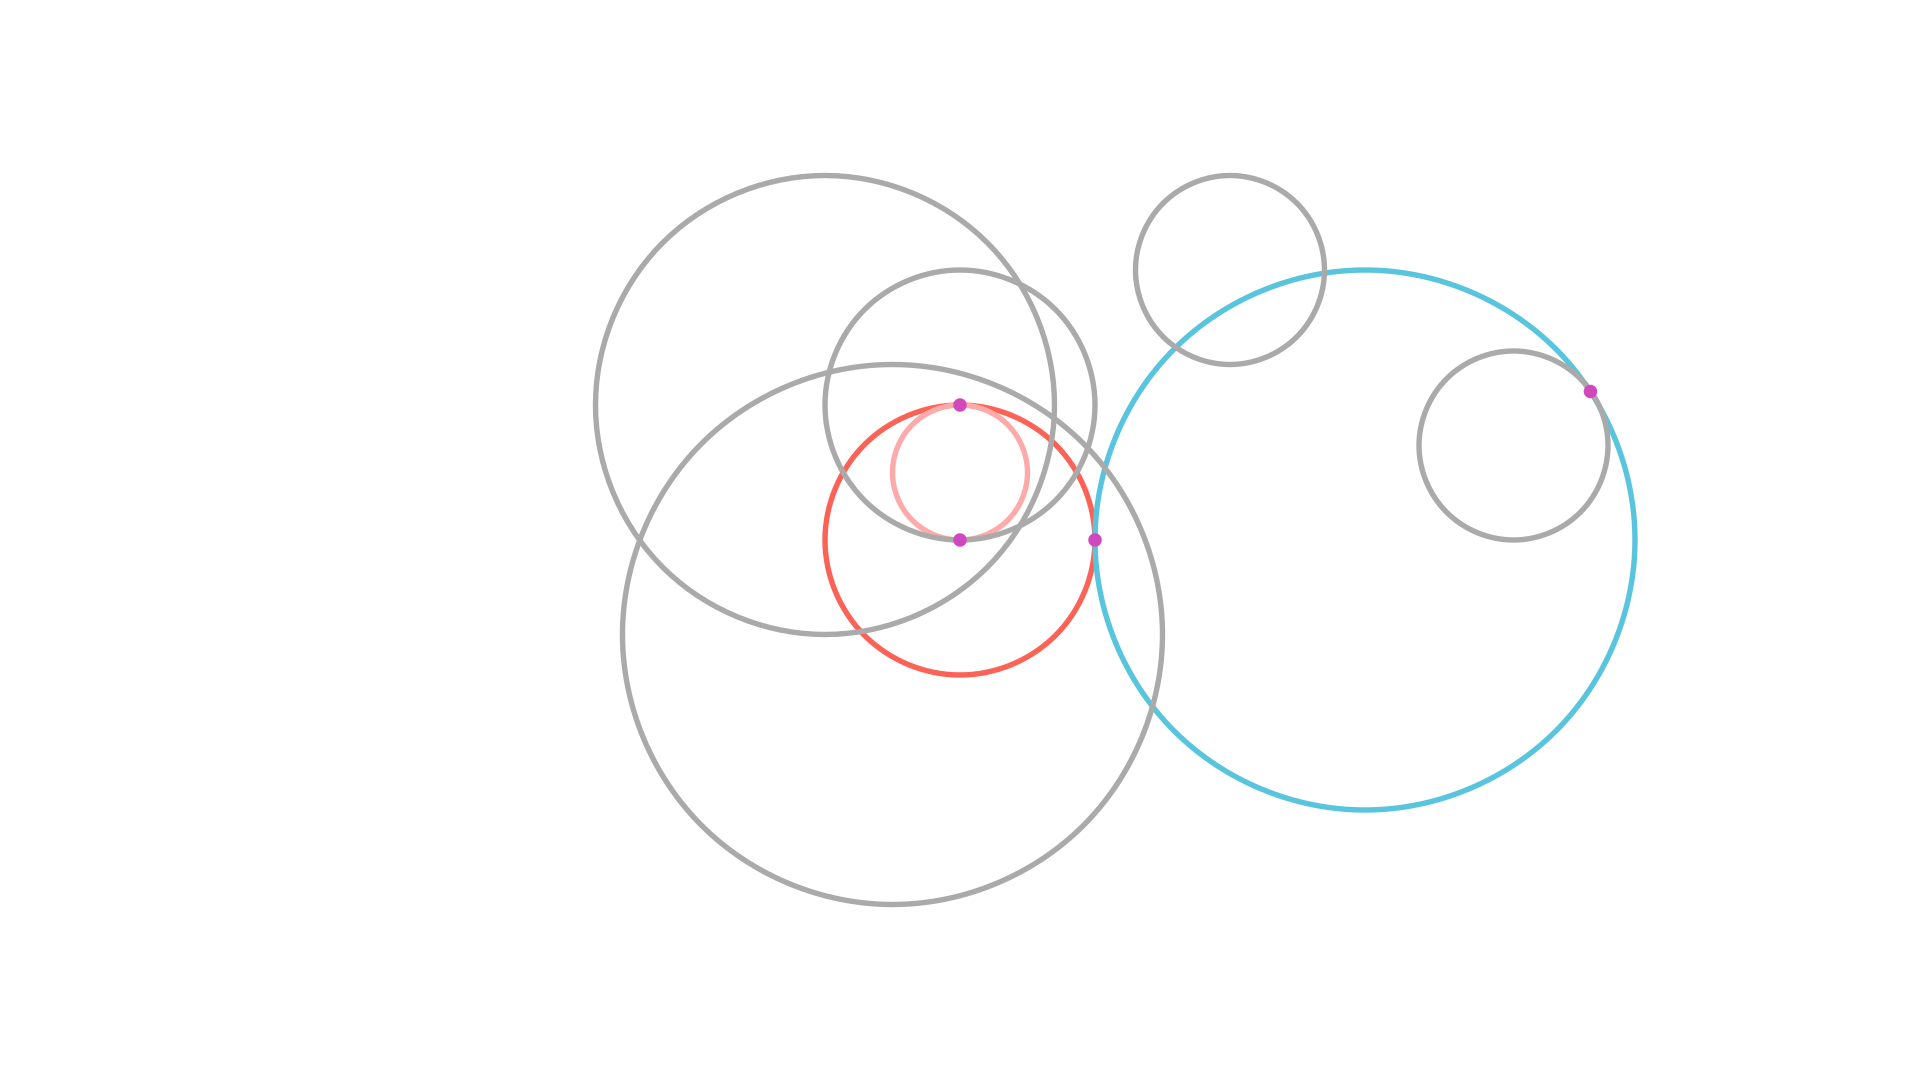
\includegraphics[trim={5cm 0 4cm 2cm}, clip,width=0.8
        \textwidth]{images/Diagram1.png}

    \end{figure}
}

\nfr{{Circle Tangencies: What's degenerate?}
Collection of $N$ circles with $\sim N^2$ tangencies:
\begin{figure}[h]
    \centering
    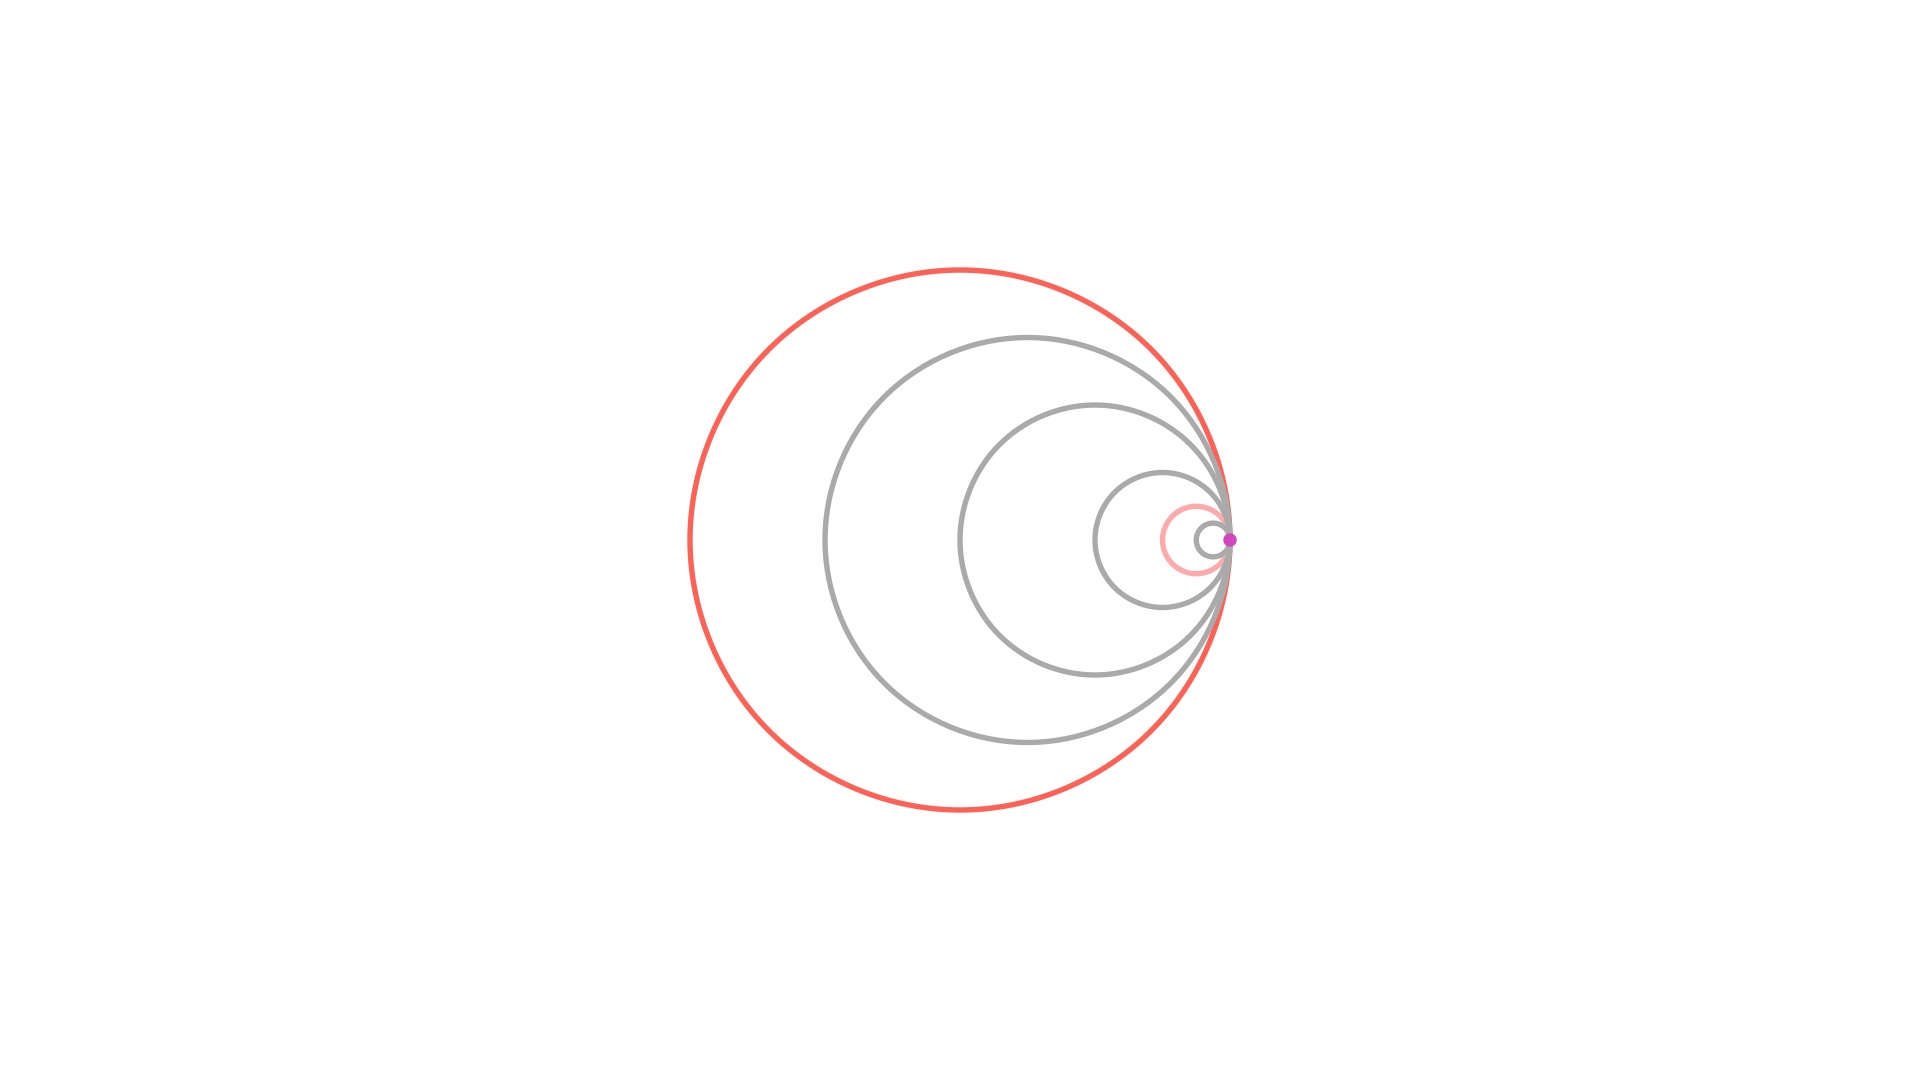
\includegraphics[width=1
    \textwidth, trim={5cm 2cm 4cm 2cm}, clip=true]{images/Diagram2.png}
\end{figure}
}


\nfr{{Circle Tangencies: Lifting into $\RR^3$}
\begin{theorem}
    Given a (suitably non-degenerate) collection of $N$ circles in $\RR^2$, they determine $\lesssim N^{3/2}$ tangencies.
\end{theorem}
We now present a sketch of a recent proof due to Ellenberg, Solymosi, and Zahl. \cite{ellenberg2016new} \pause

\textbf{Sketch Proof:}
Assume:
\begin{itemize}
    \item There are $\gtrsim N^{3/2}$ tangencies.
    \item Collection is uniform: each circle tangent to $\gtrsim N^{1/2}$ other circles.
\end{itemize}
For each circle $\gamma$ in our collection, we define the curve $\beta(\gamma) \subset \RR^3$ as: \[\beta(\gamma) := \left\{(x,y,z) \ | \ (x,y) \in \gamma,\ z = \frac{1}{\text{Slope of tangent at }(x,y)} \right\}
\]


}

\nfr{{Circle Tangencies: Lifting into $\RR^3$}

\begin{figure}[h]
    \centering
    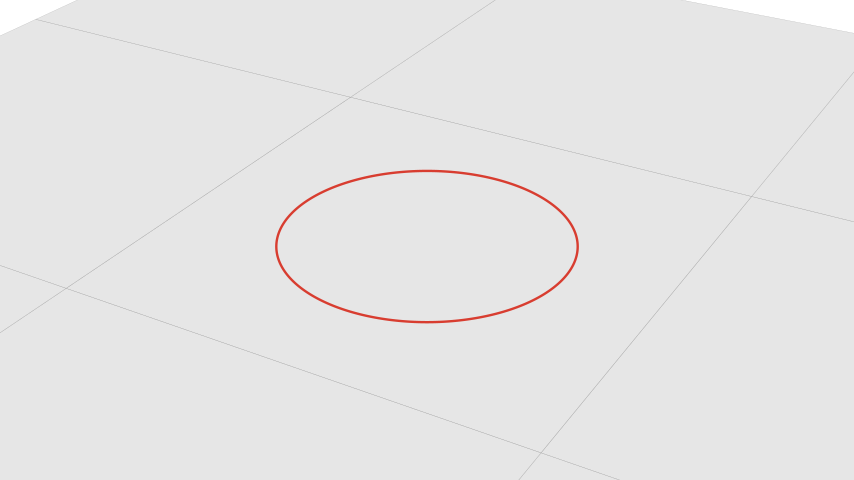
\includegraphics[width=0.8
    \textwidth, trim={5cm 0 4cm 2cm}, clip=true]{images/Diagram3a.png}
\end{figure}
}


\nfr{{Circle Tangencies: Lifting into $\RR^3$}

\begin{figure}[h]
    \centering
    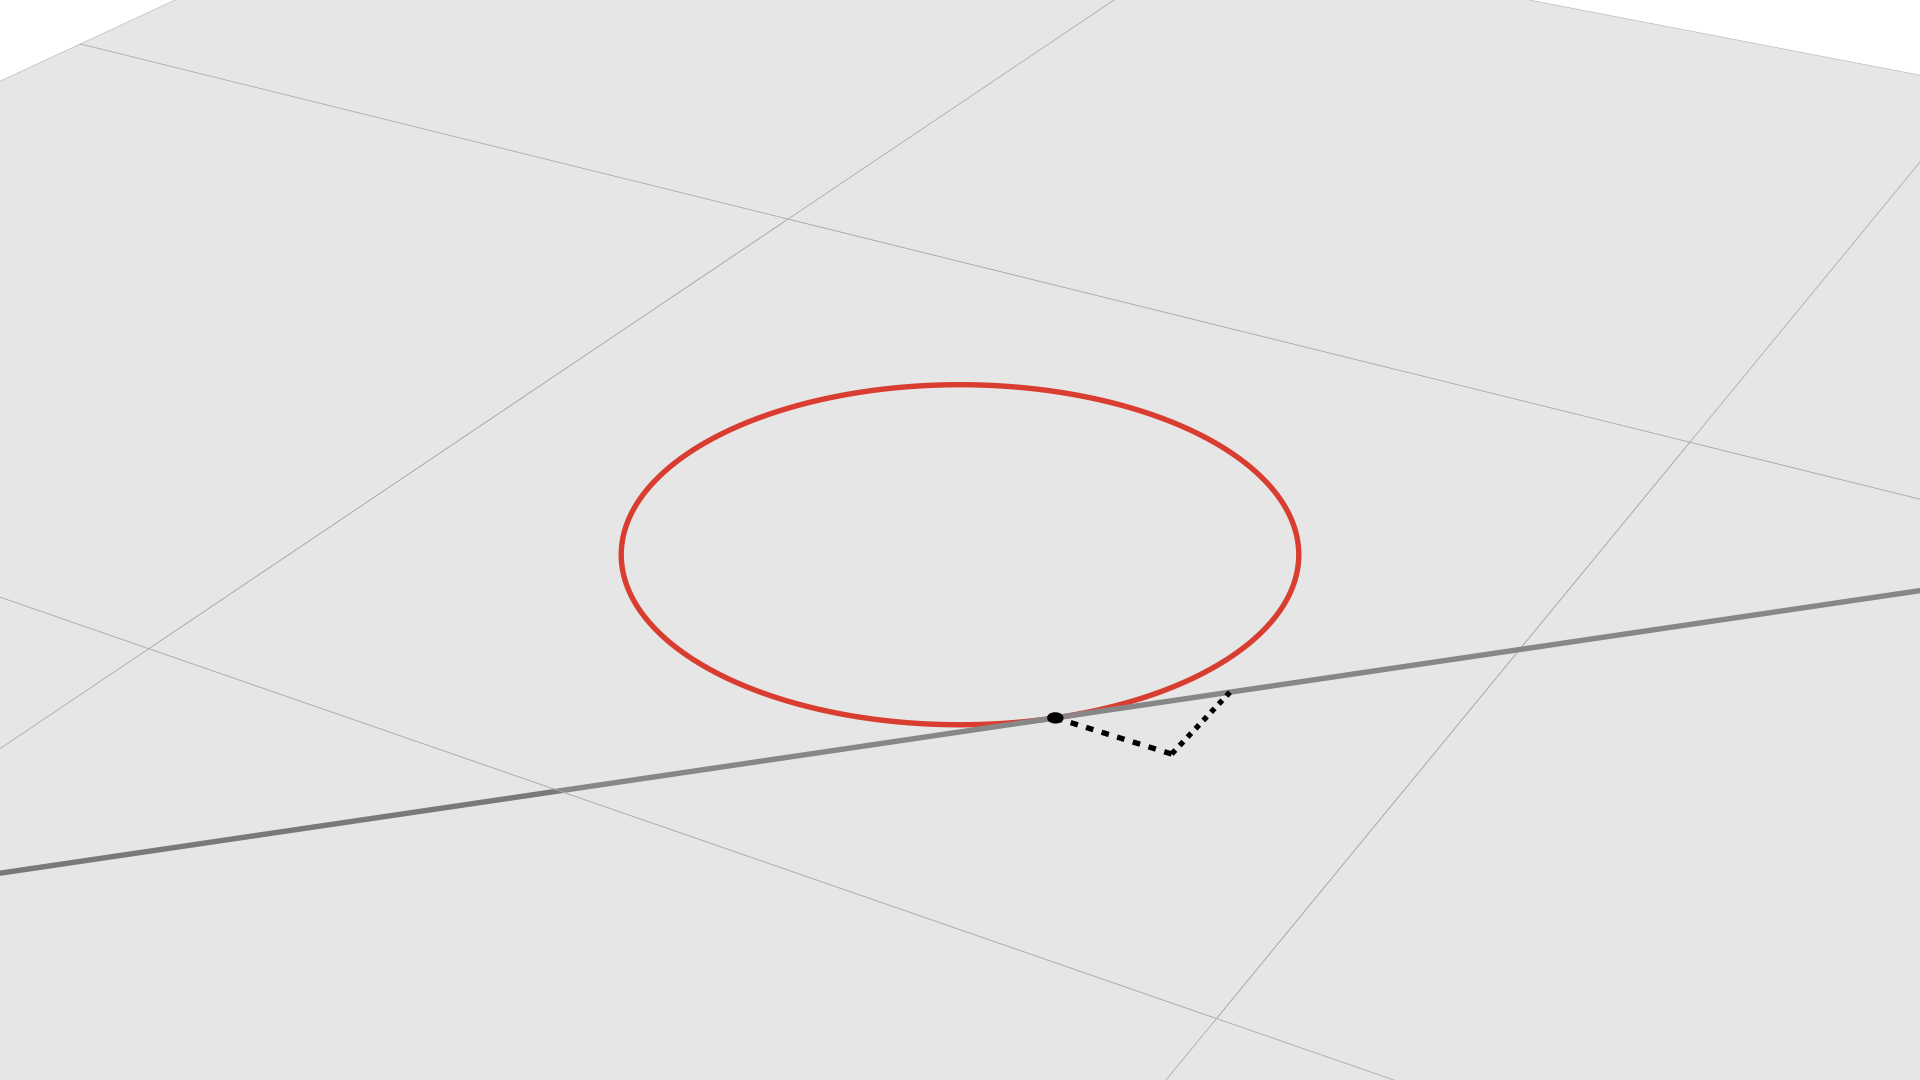
\includegraphics[width=0.8
    \textwidth, trim={5cm 0 4cm 2cm}, clip=true]{images/Diagram3b.png}
\end{figure}

}
\nfr{{Circle Tangencies: Lifting into $\RR^3$}
\begin{figure}[h]
    \centering
    \begin{tikzpicture}
        \node[anchor=south west,inner sep=0] (image) at (0,0) {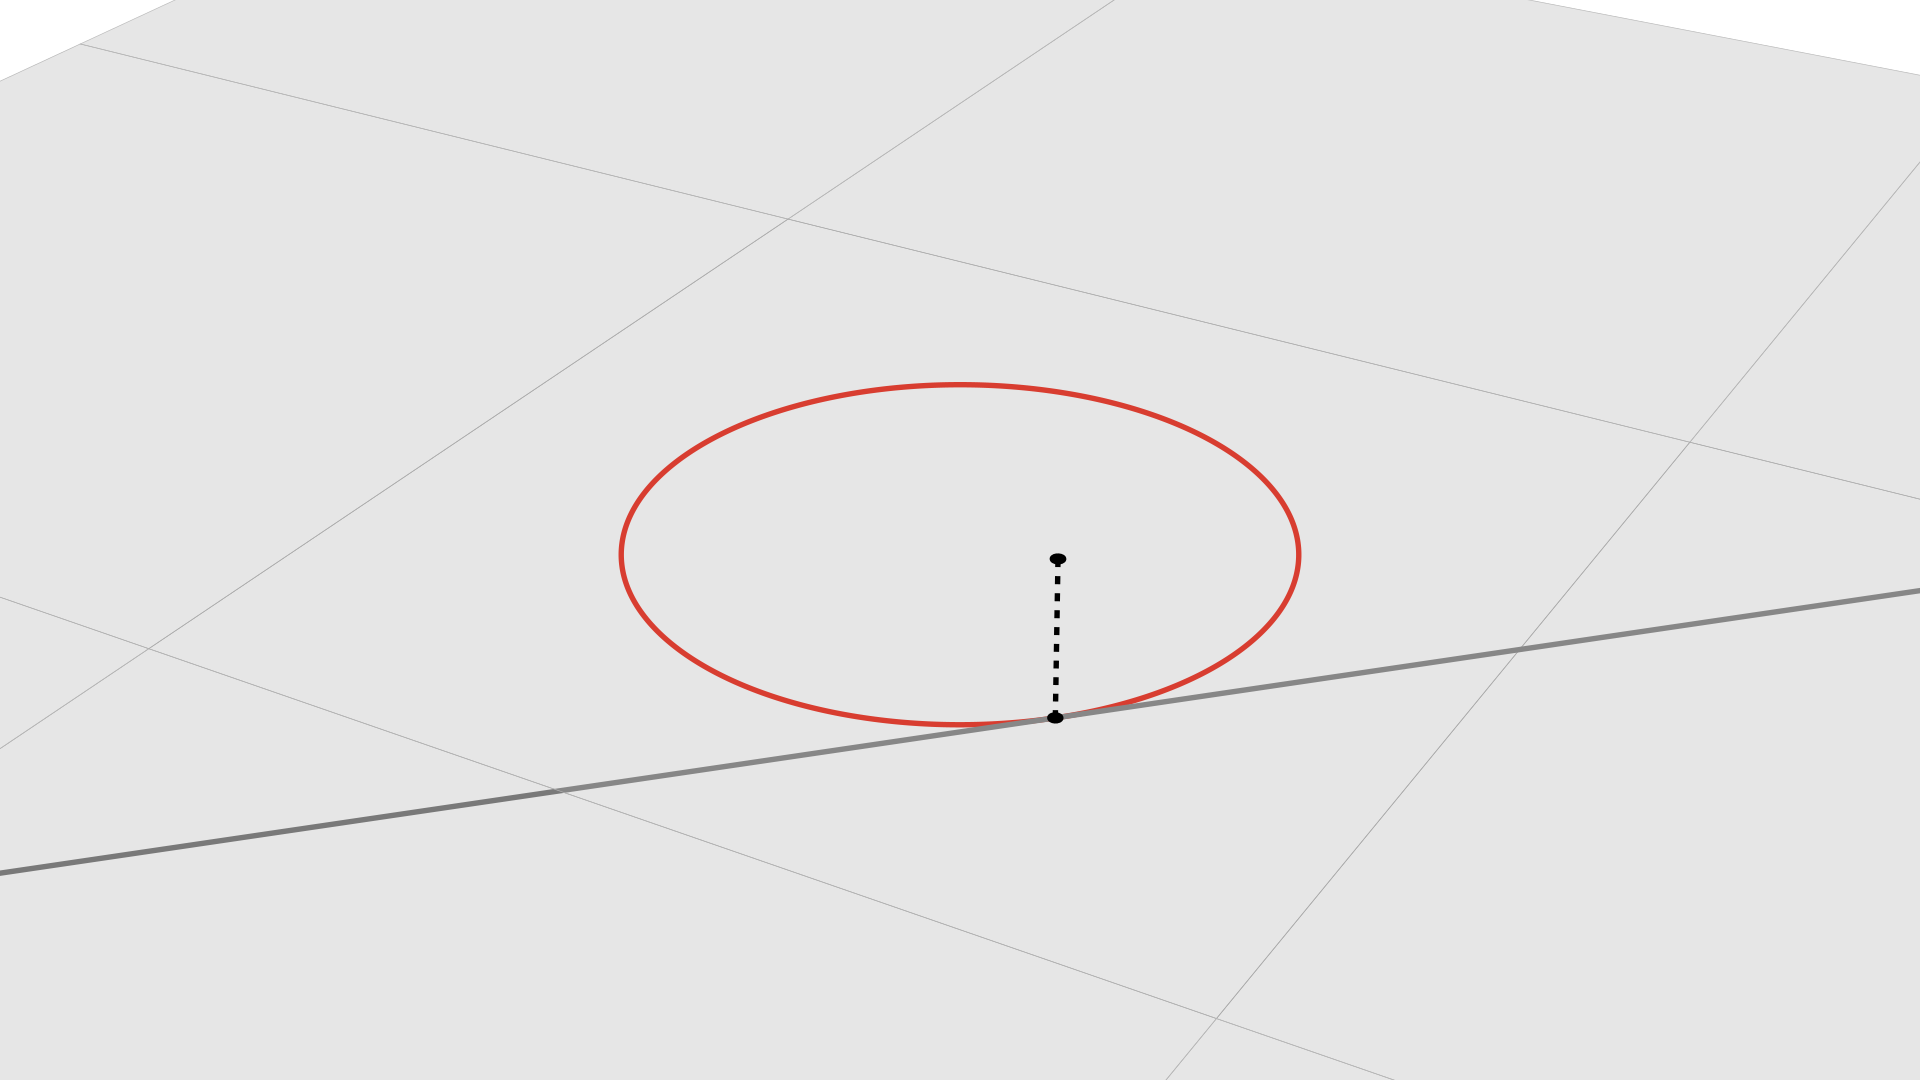
\includegraphics[width=0.8
        \textwidth, trim={5cm 0 4cm 2cm}, clip=true]{images/Diagram3c.png}};
        \begin{scope}[x={(image.south east)},y={(image.north west)}]
        \draw [decorate,
        decoration = {calligraphic brace}] (0.56,0.5) --  (0.56,0.35)
        node[pos=0.25,right=5pt,black]{$\frac{1}{\text{slope}}$};
        \end{scope}
    \end{tikzpicture}
\end{figure}
}

\nfr{{Circle Tangencies: Lifting into $\RR^3$}

\begin{figure}[h]
    \centering
    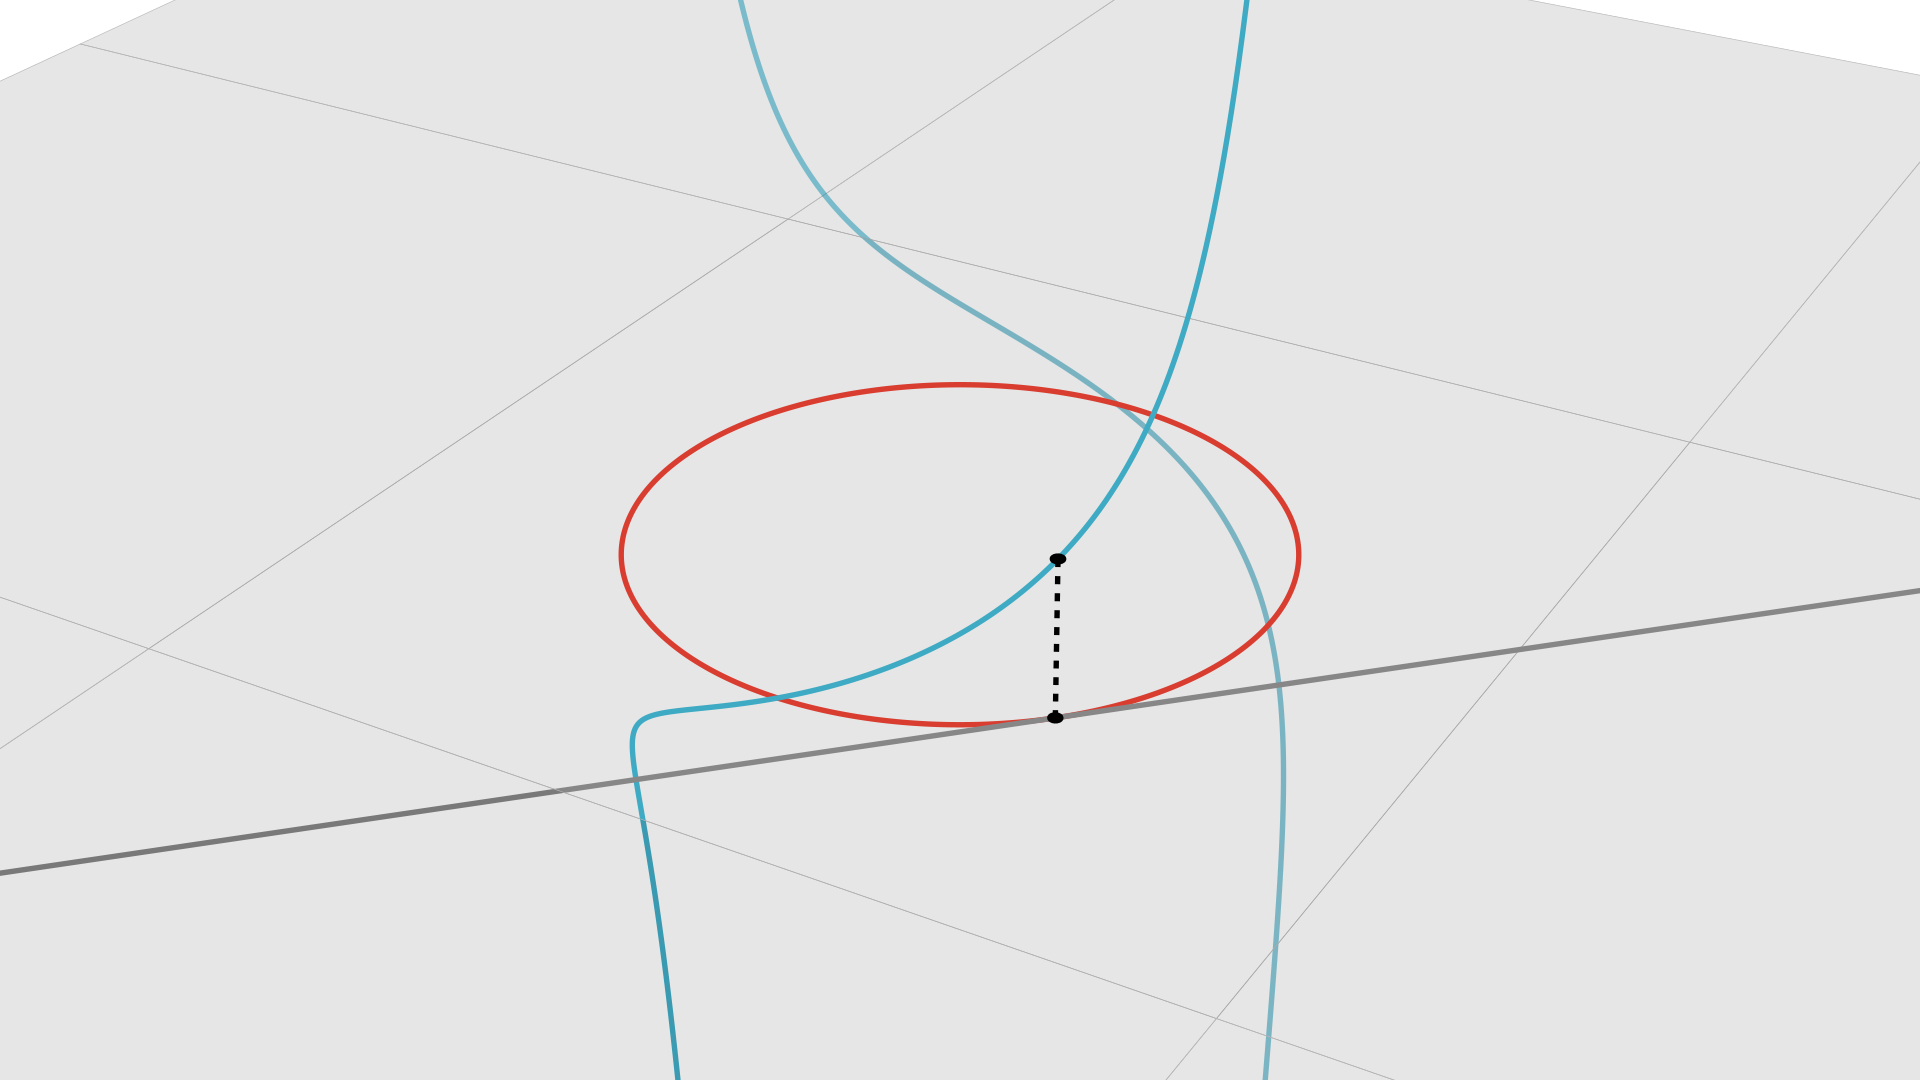
\includegraphics[width=0.8
    \textwidth, trim={5cm 0 4cm 2cm}, clip=true]{images/Diagram3d.png}
\end{figure}

}




\nfr{{Circle Tangencies: Tangencies to Incidences}

\begin{figure}[h]
    \centering
    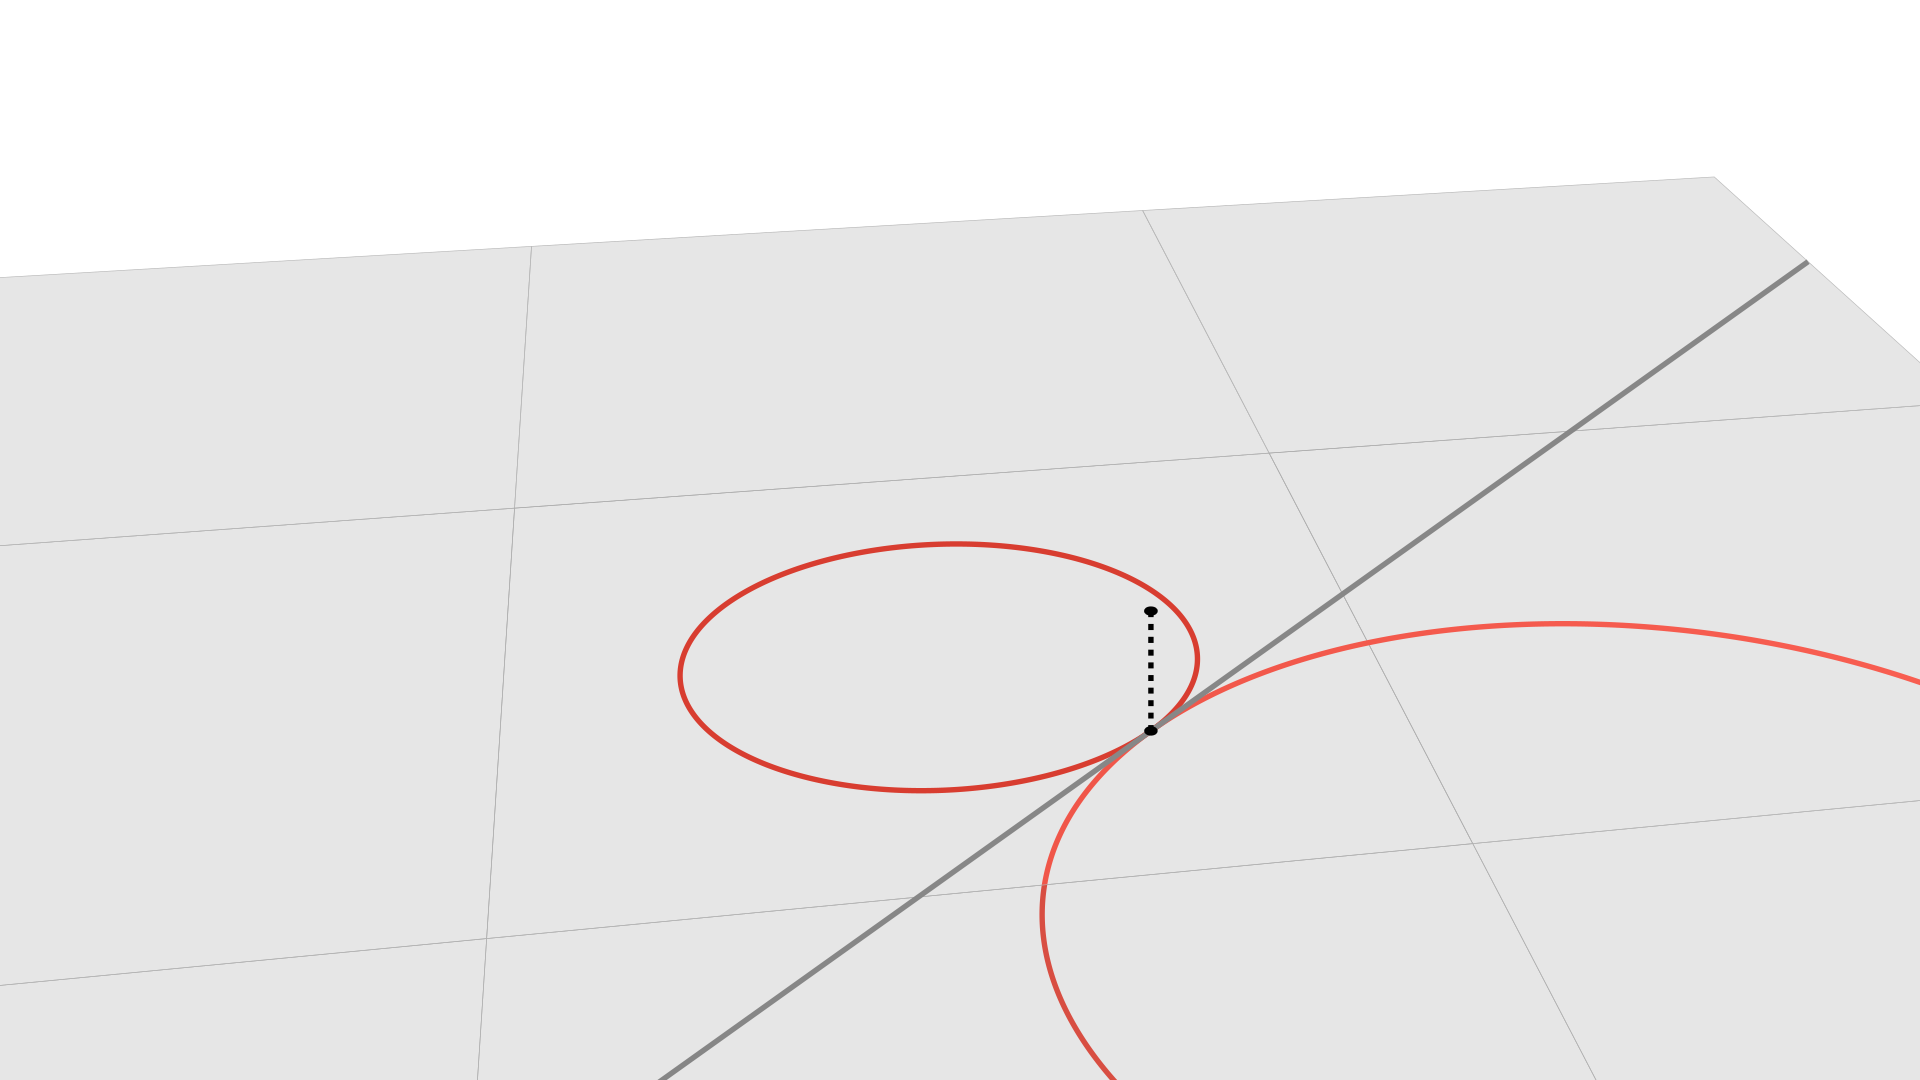
\includegraphics[width=0.8
    \textwidth, trim={5cm 0 4cm 2cm}, clip=true]{images/Diagram4a.png}
\end{figure}


}

\nfr{{Circle Tangencies: Tangencies to Incidences}

\begin{figure}[h]
    \centering
    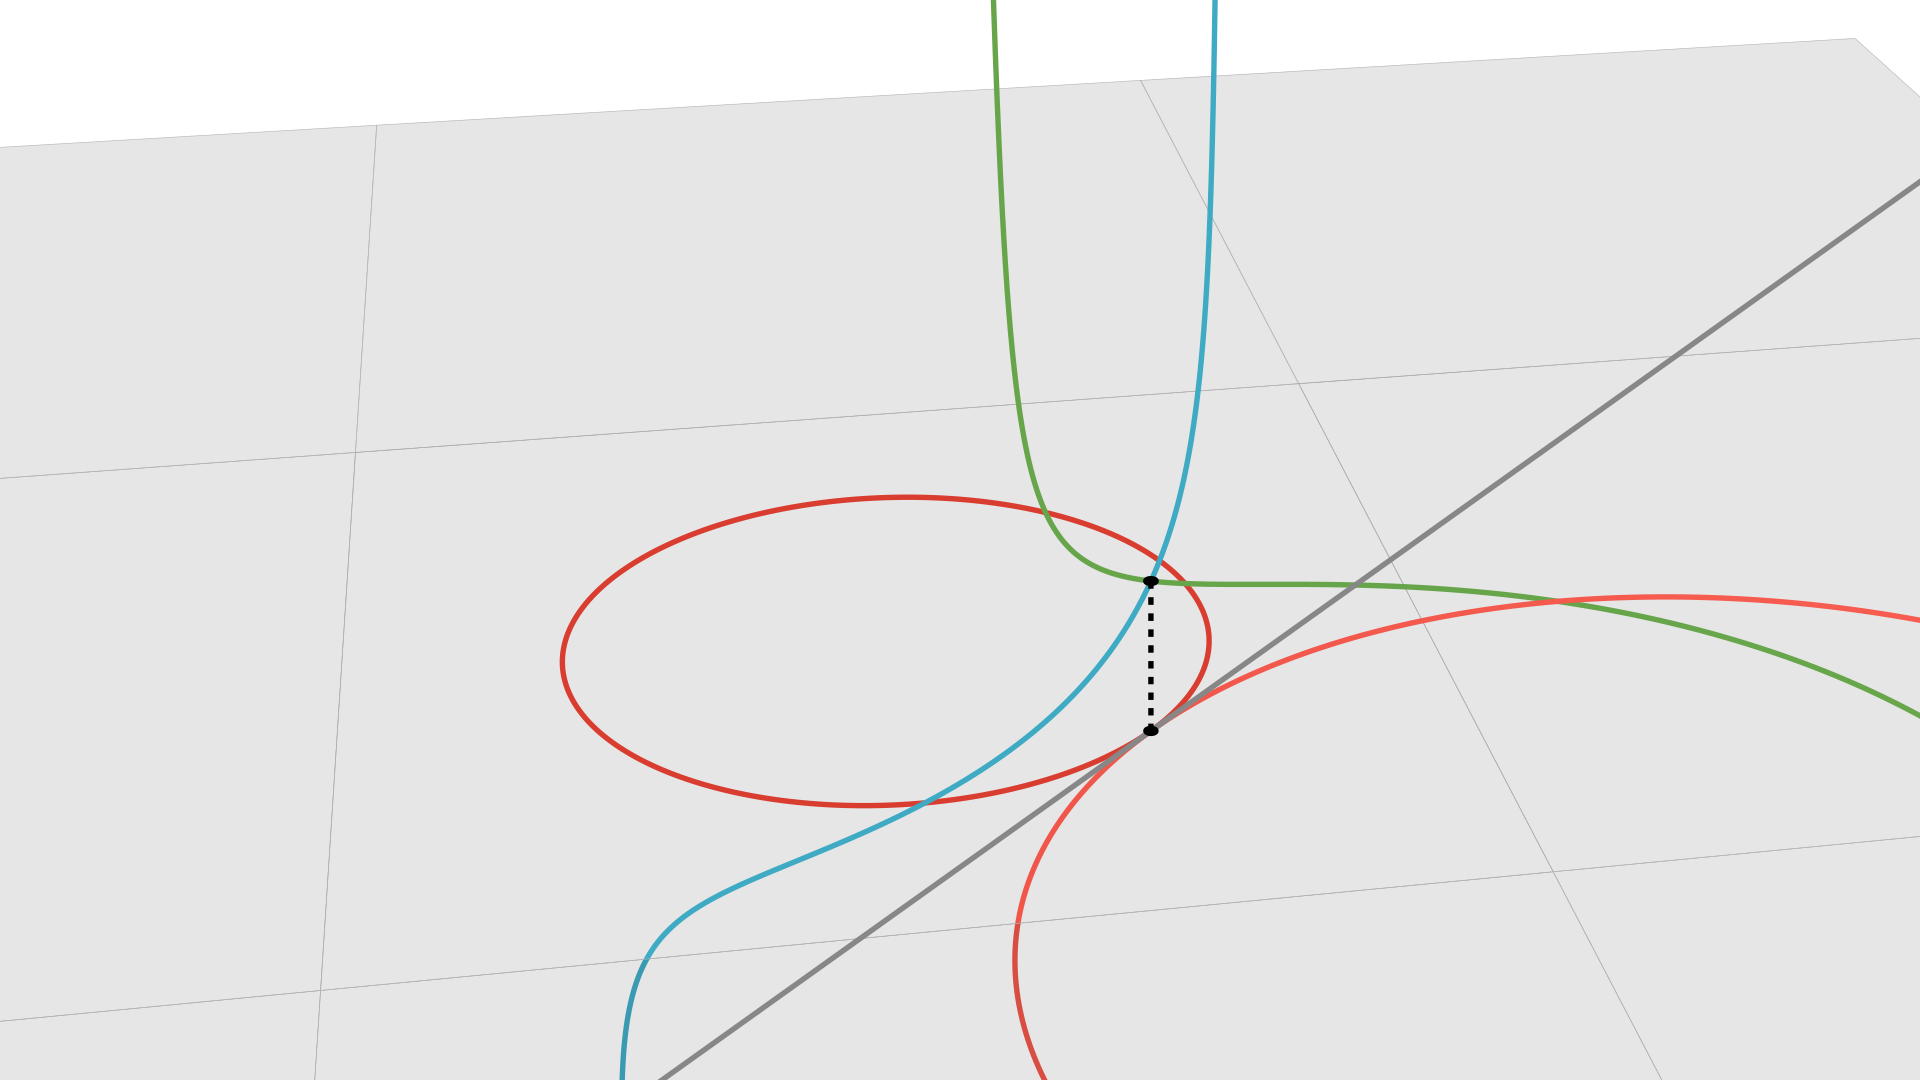
\includegraphics[width=0.8
    \textwidth, trim={5cm 0 4cm 2cm}, clip=true]{images/Diagram4b.png}
\end{figure}
Intersection  $\implies z$ co-ords equal $\implies$  circles are tangent.

Tangency problem in $\RR^2 \iff $ Incidences problem in $\RR^3$.
}

\nfr{{Circle Tangencies: Tangencies to Incidences}

\begin{figure}[h]
    \centering
    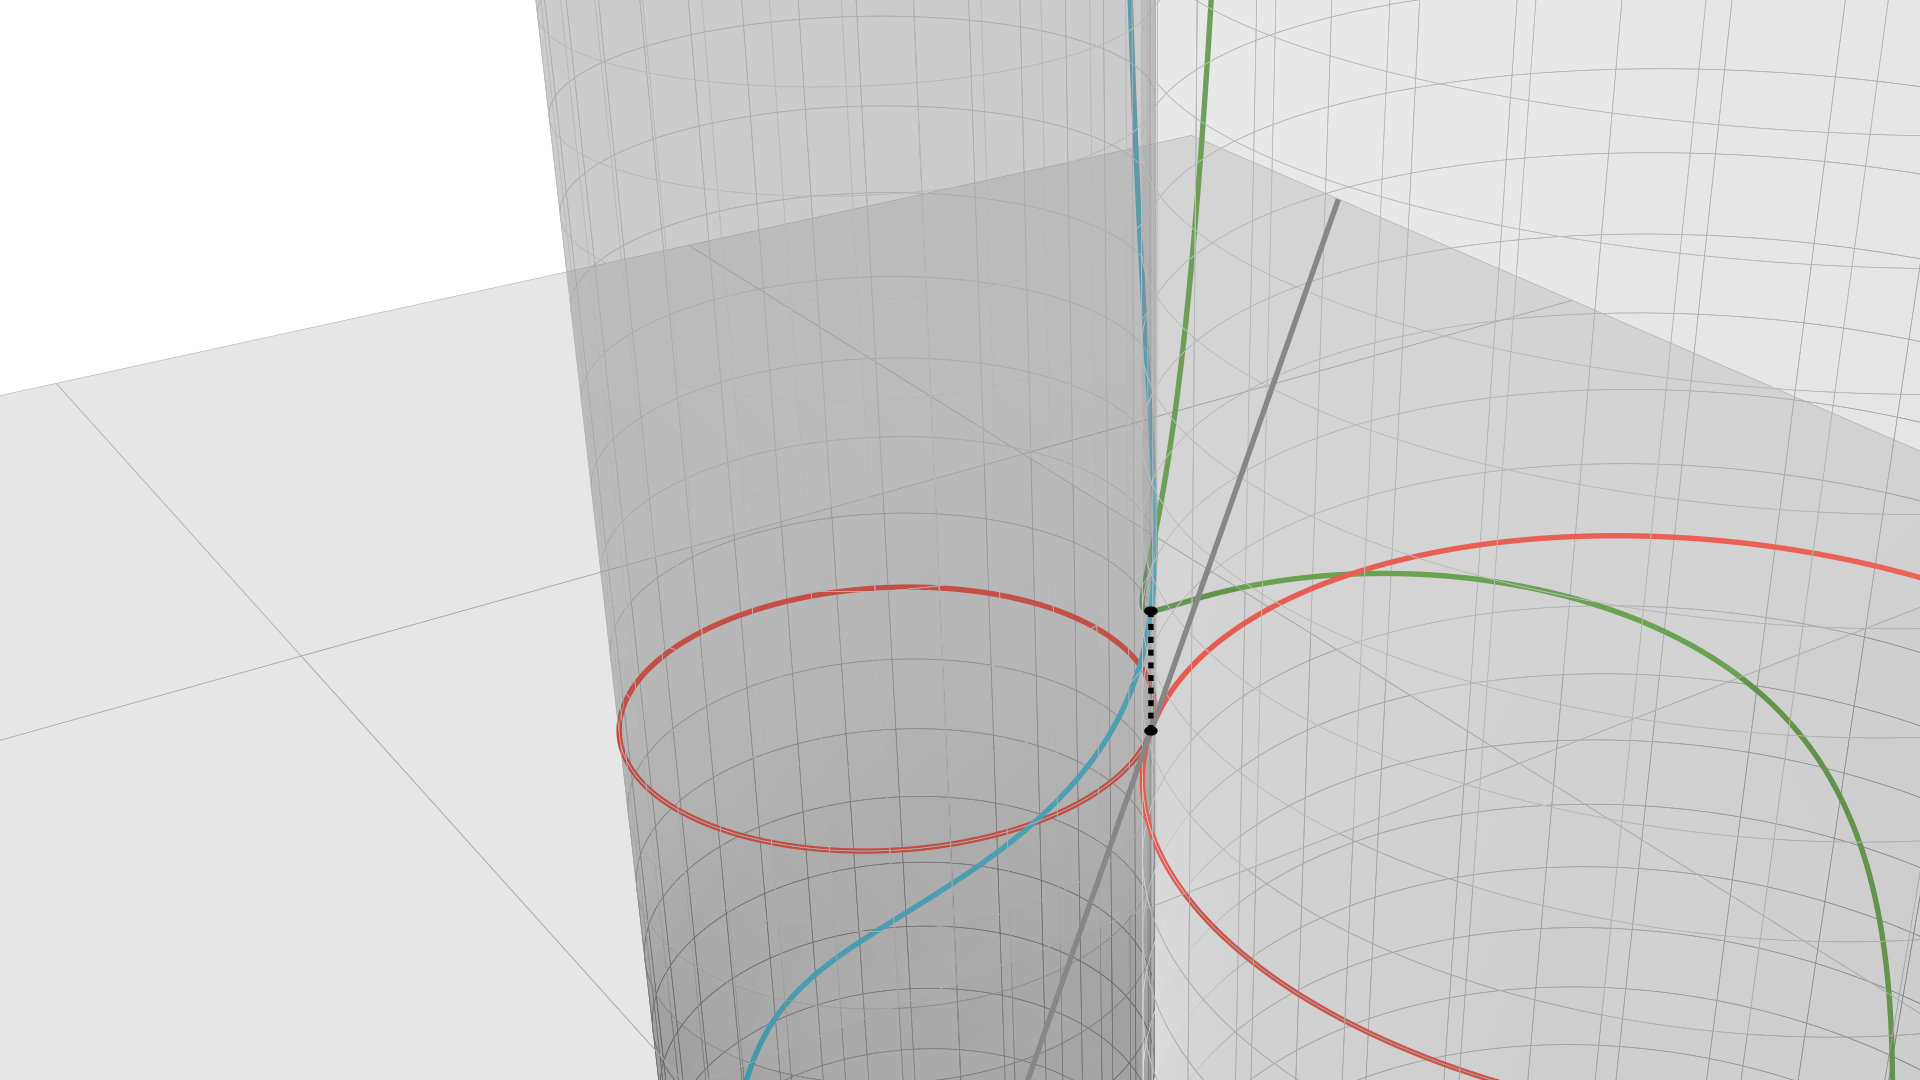
\includegraphics[width=0.8
    \textwidth, trim={5cm 0 4cm 2cm}, clip=true]{images/Diagram4c.png}
\end{figure}

Intersection  $\implies z$ co-ords equal $\implies$  circles are tangent.

Tangency problem in $\RR^2 \iff $ Incidences problem in $\RR^3$.
}

\nfr{{Circle Tangencies: Tangent Vectors at Incidences}
Let us examine the tangent vectors at a point of incidence between two curves:
\begin{figure}[h]
    \centering
    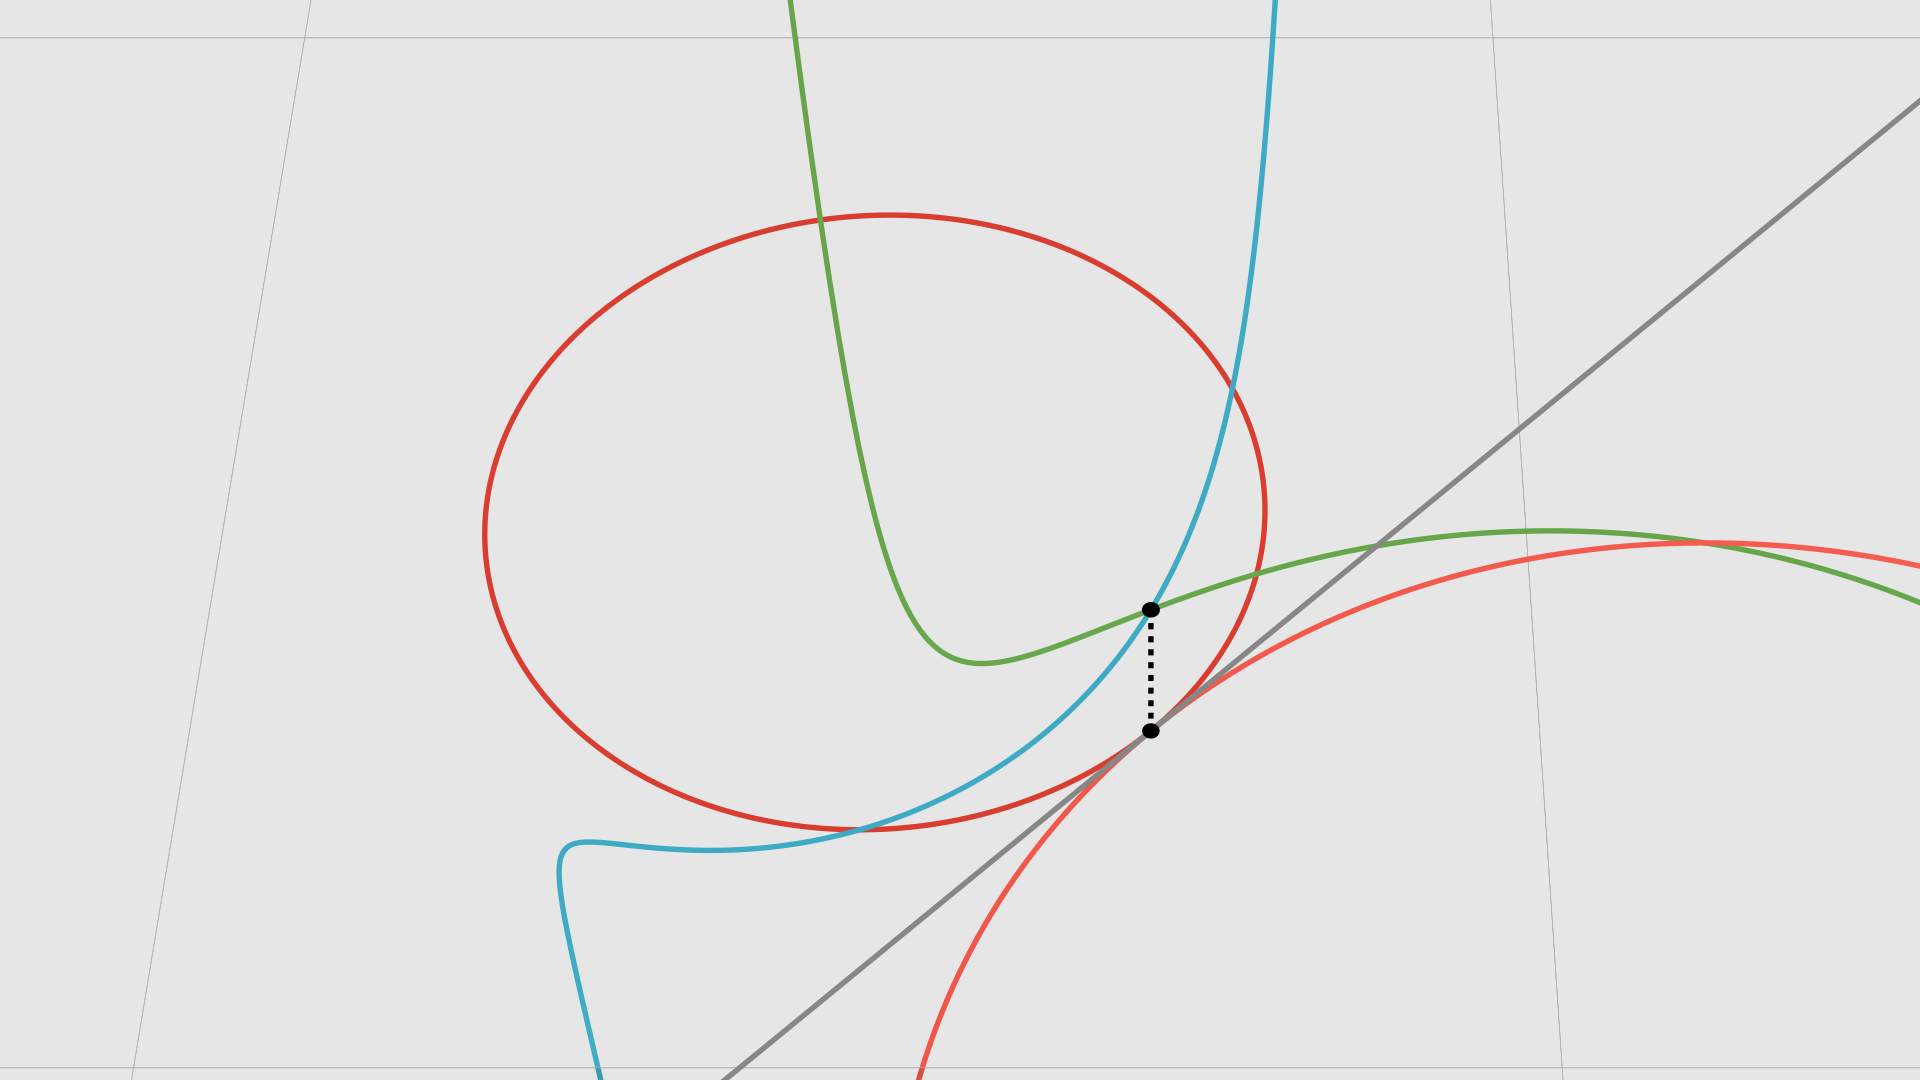
\includegraphics[width=0.8
    \textwidth, trim={5cm 0 4cm 2cm}, clip=true]{images/Diagram5a.png}
\end{figure}

}
\nfr{{Circle Tangencies: Tangent Vectors at Incidences}

\begin{figure}[h]
    \centering
    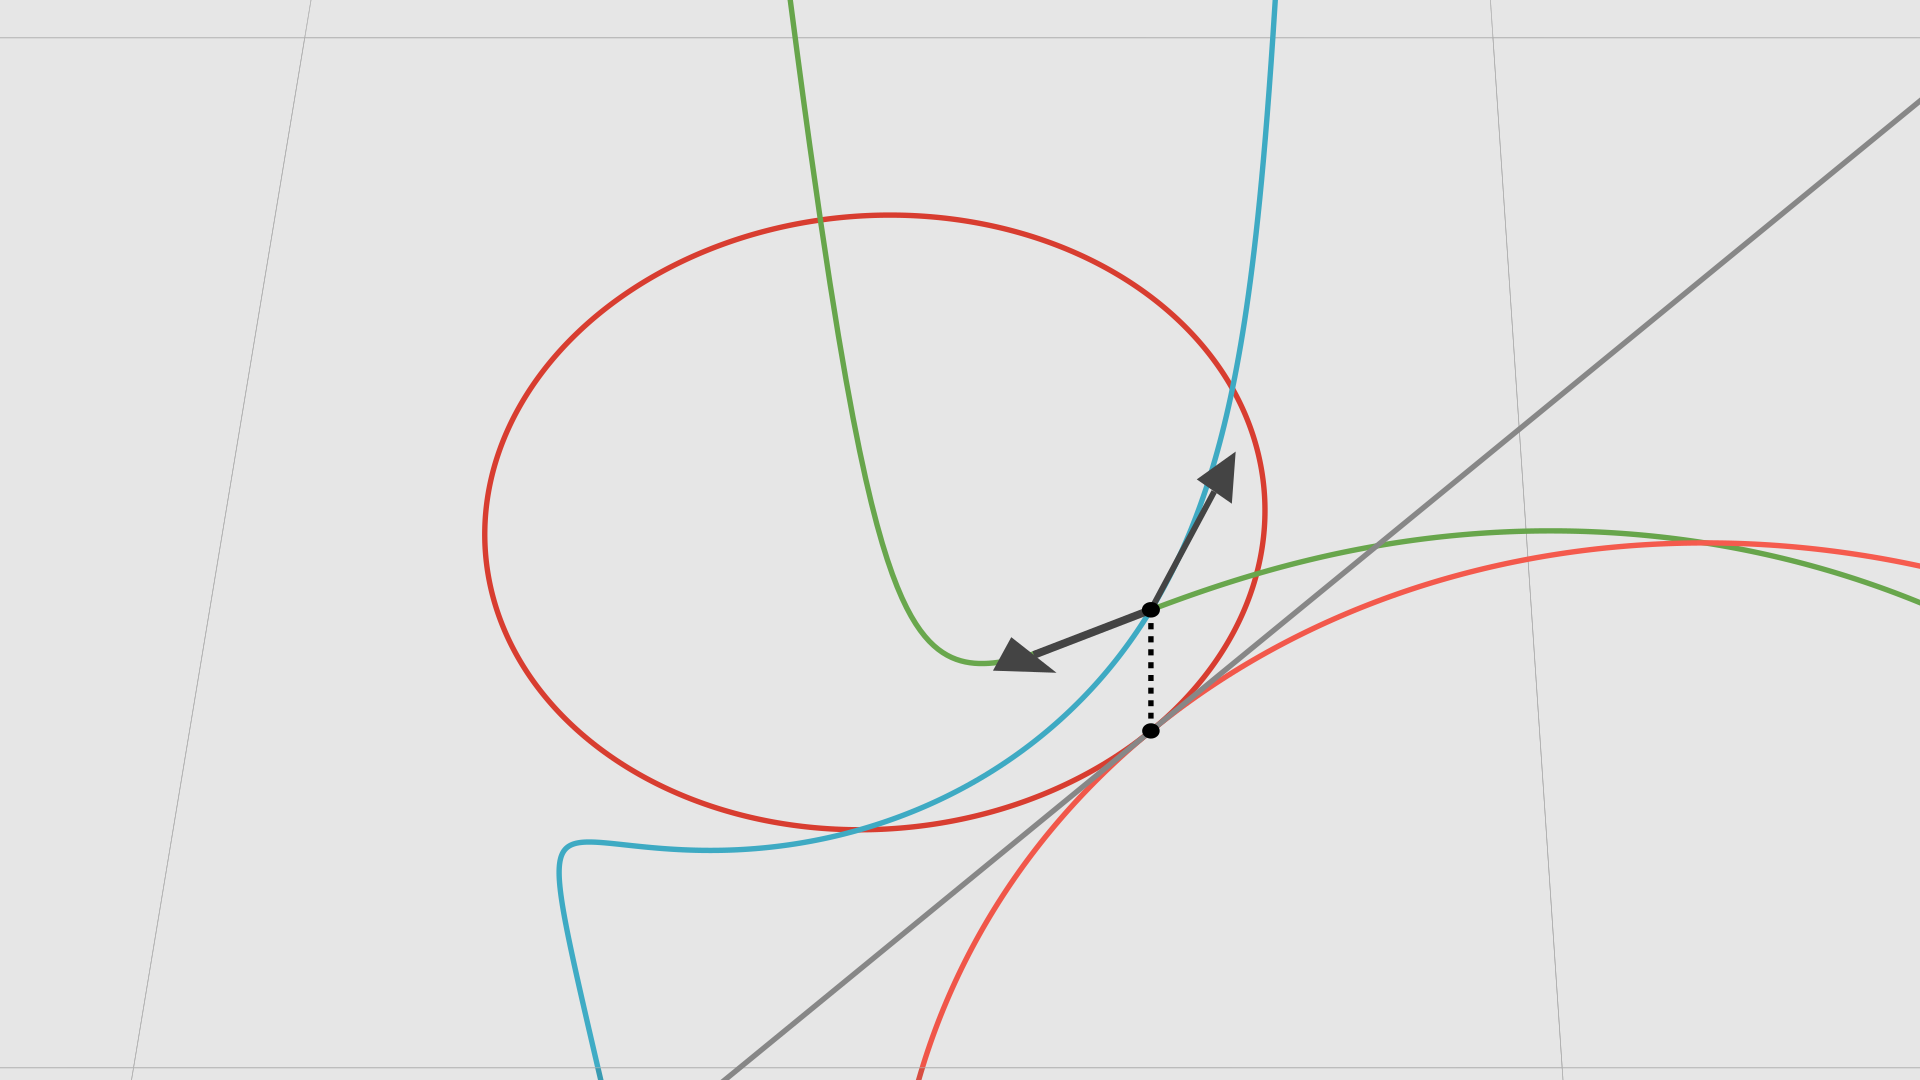
\includegraphics[width=0.8
    \textwidth, trim={5cm 0 4cm 2cm}, clip=true]{images/Diagram5b.png}
\end{figure} \pause
At every point of intersection, the tangent vectors span a vertical plane. 
}
\nfr{{Circle Tangencies: Tangent Vectors at Incidences}

\begin{figure}[h]
    \centering
    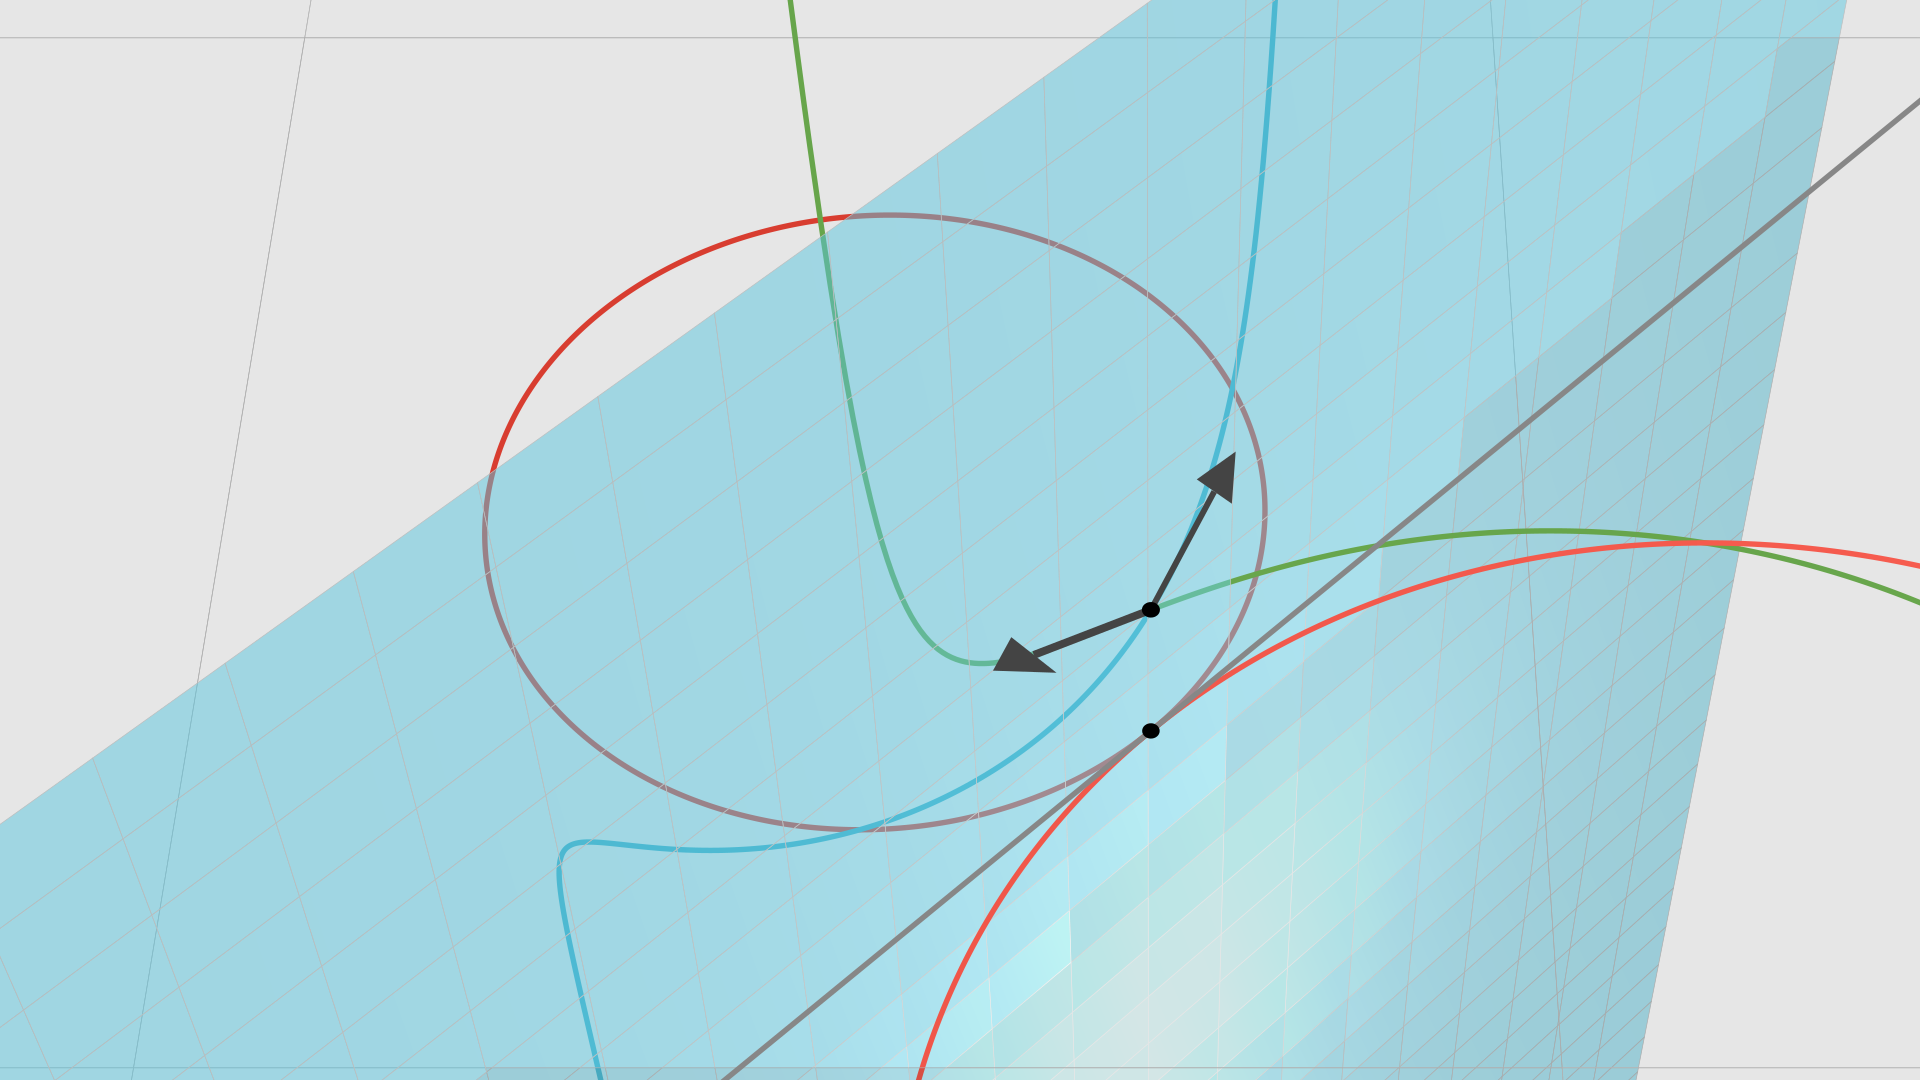
\includegraphics[width=0.8
    \textwidth, trim={5cm 0 4cm 2cm}, clip=true]{images/Diagram5c.png}
\end{figure}

At every point of intersection, the tangent vectors span a vertical plane. 

}



\nfr{{Circle Tangencies: Interpolation}
Let $P$ be a polynomial such that all $N^{3/2}$ incidences are contained in $Z(P)$. 

\begin{figure}[h]
    \centering
    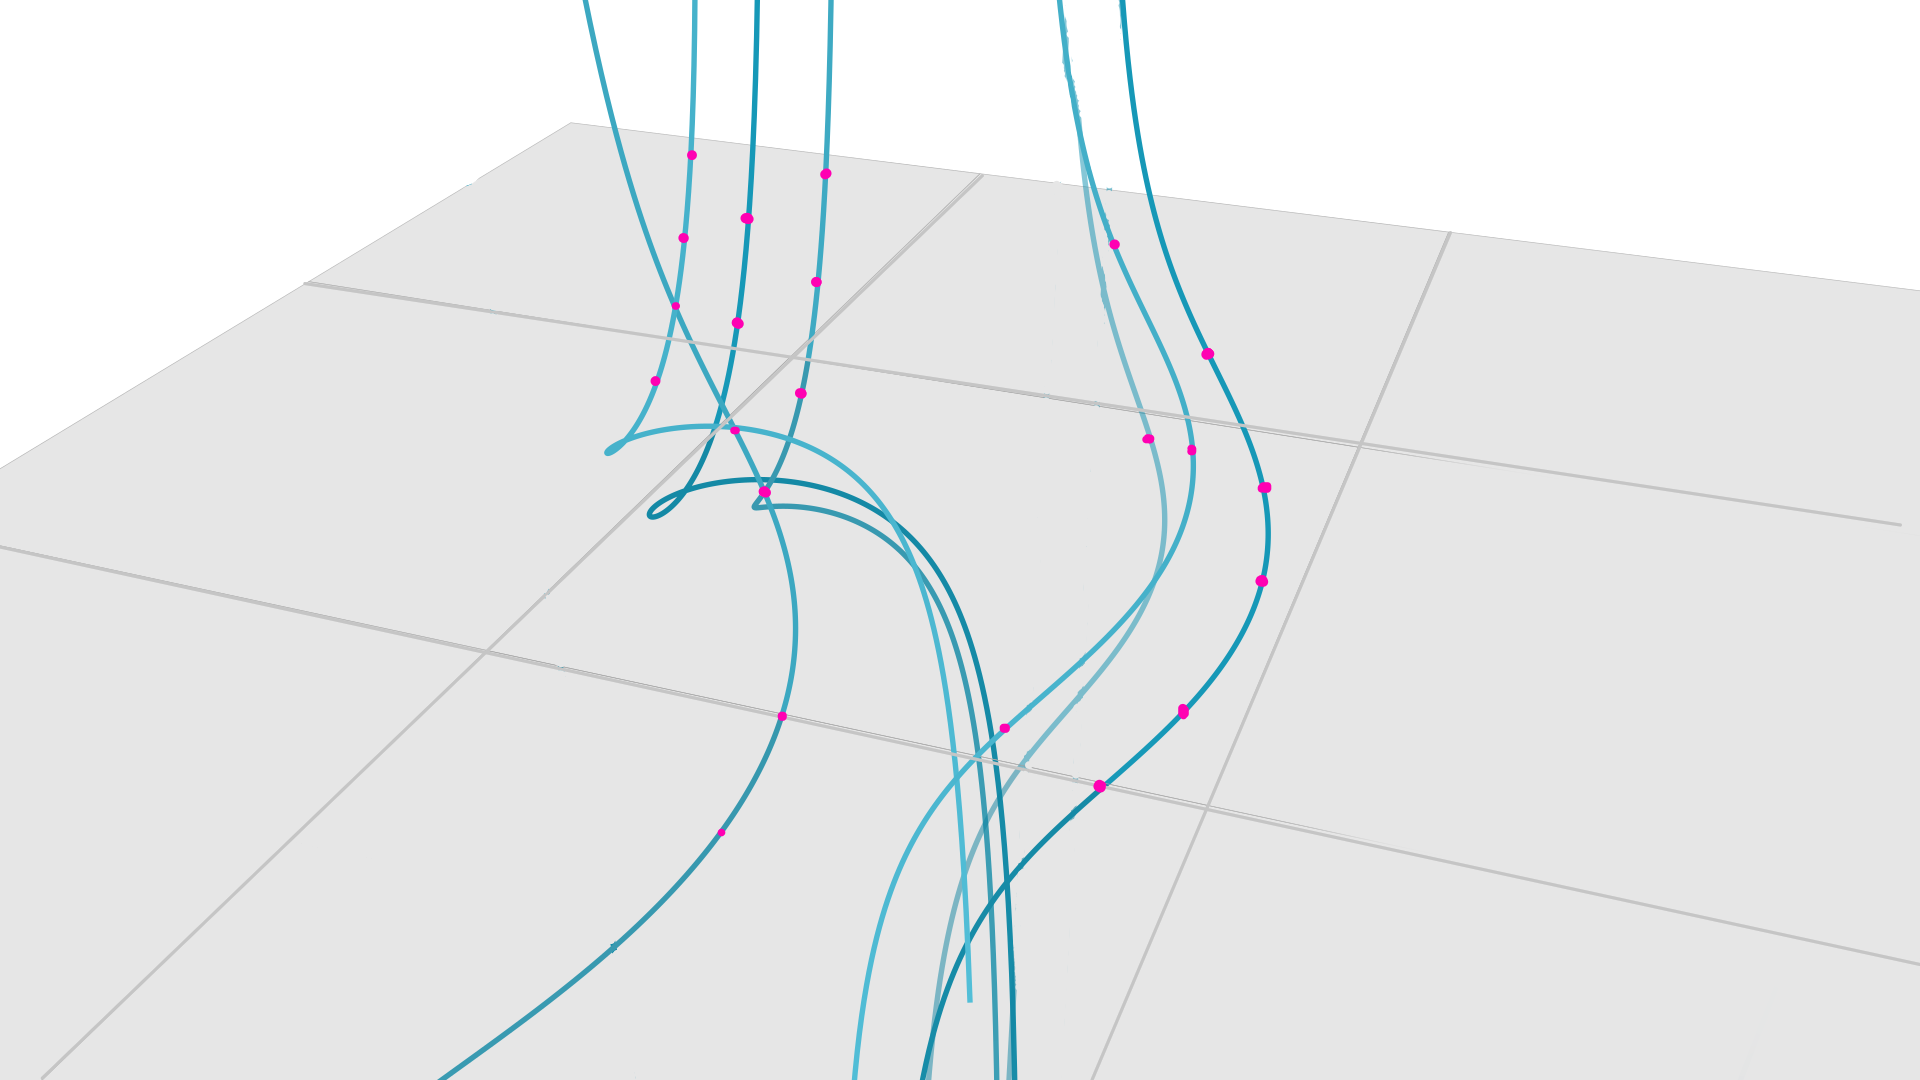
\includegraphics[width=0.7\textwidth]{images/lots_of_dots_a.png}
\end{figure}
}
\nfr{{Circle Tangencies: Interpolation}
We can find a polynomial $P$ such that all $N^{3/2}$ incidences are contained in $Z(P)$. 

\begin{figure}[h]
    \centering
    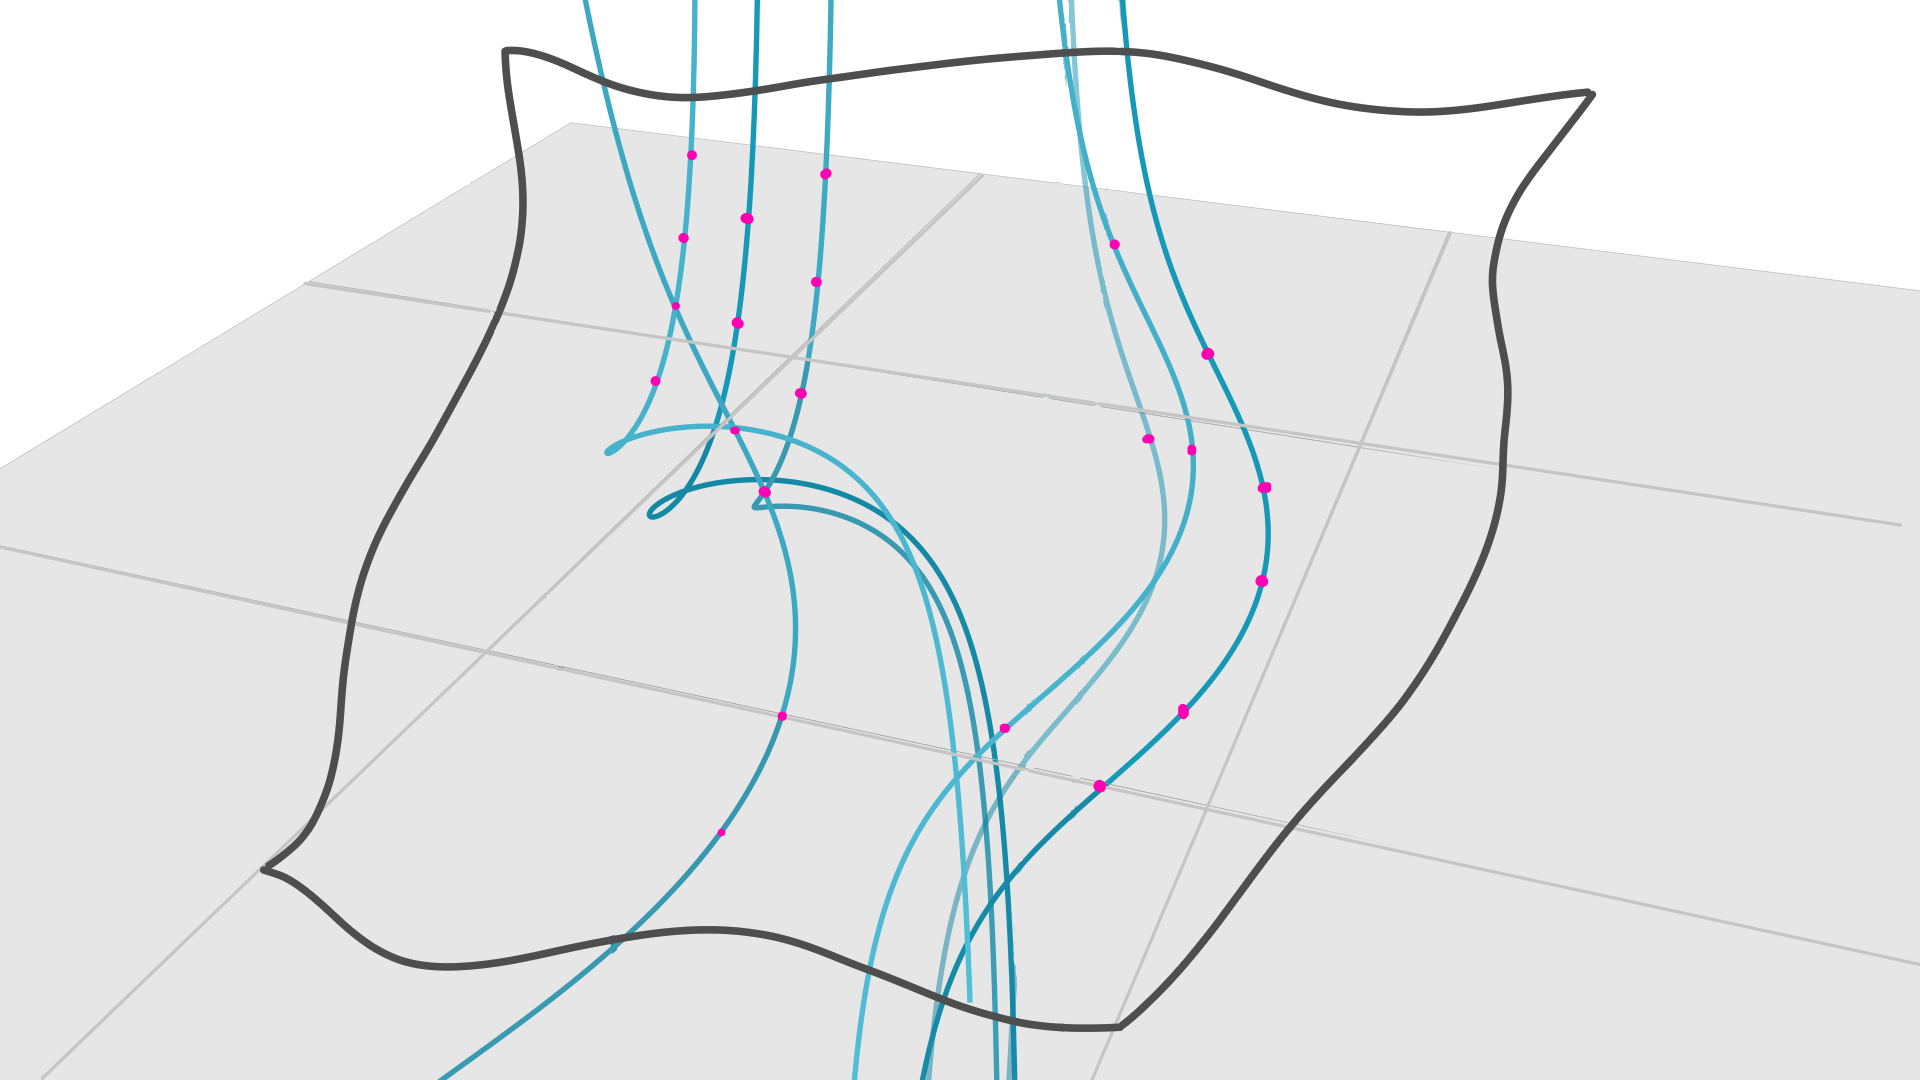
\includegraphics[width=0.7\textwidth]{images/lots_of_dots_b.png}
\end{figure}
}



\nfr{{Circle Tangencies: Interpolation}
Let $P$ be a polynomial such that all $N^{3/2}$ incidences are contained in $Z(P)$. 

\begin{figure}[h]
    \centering
    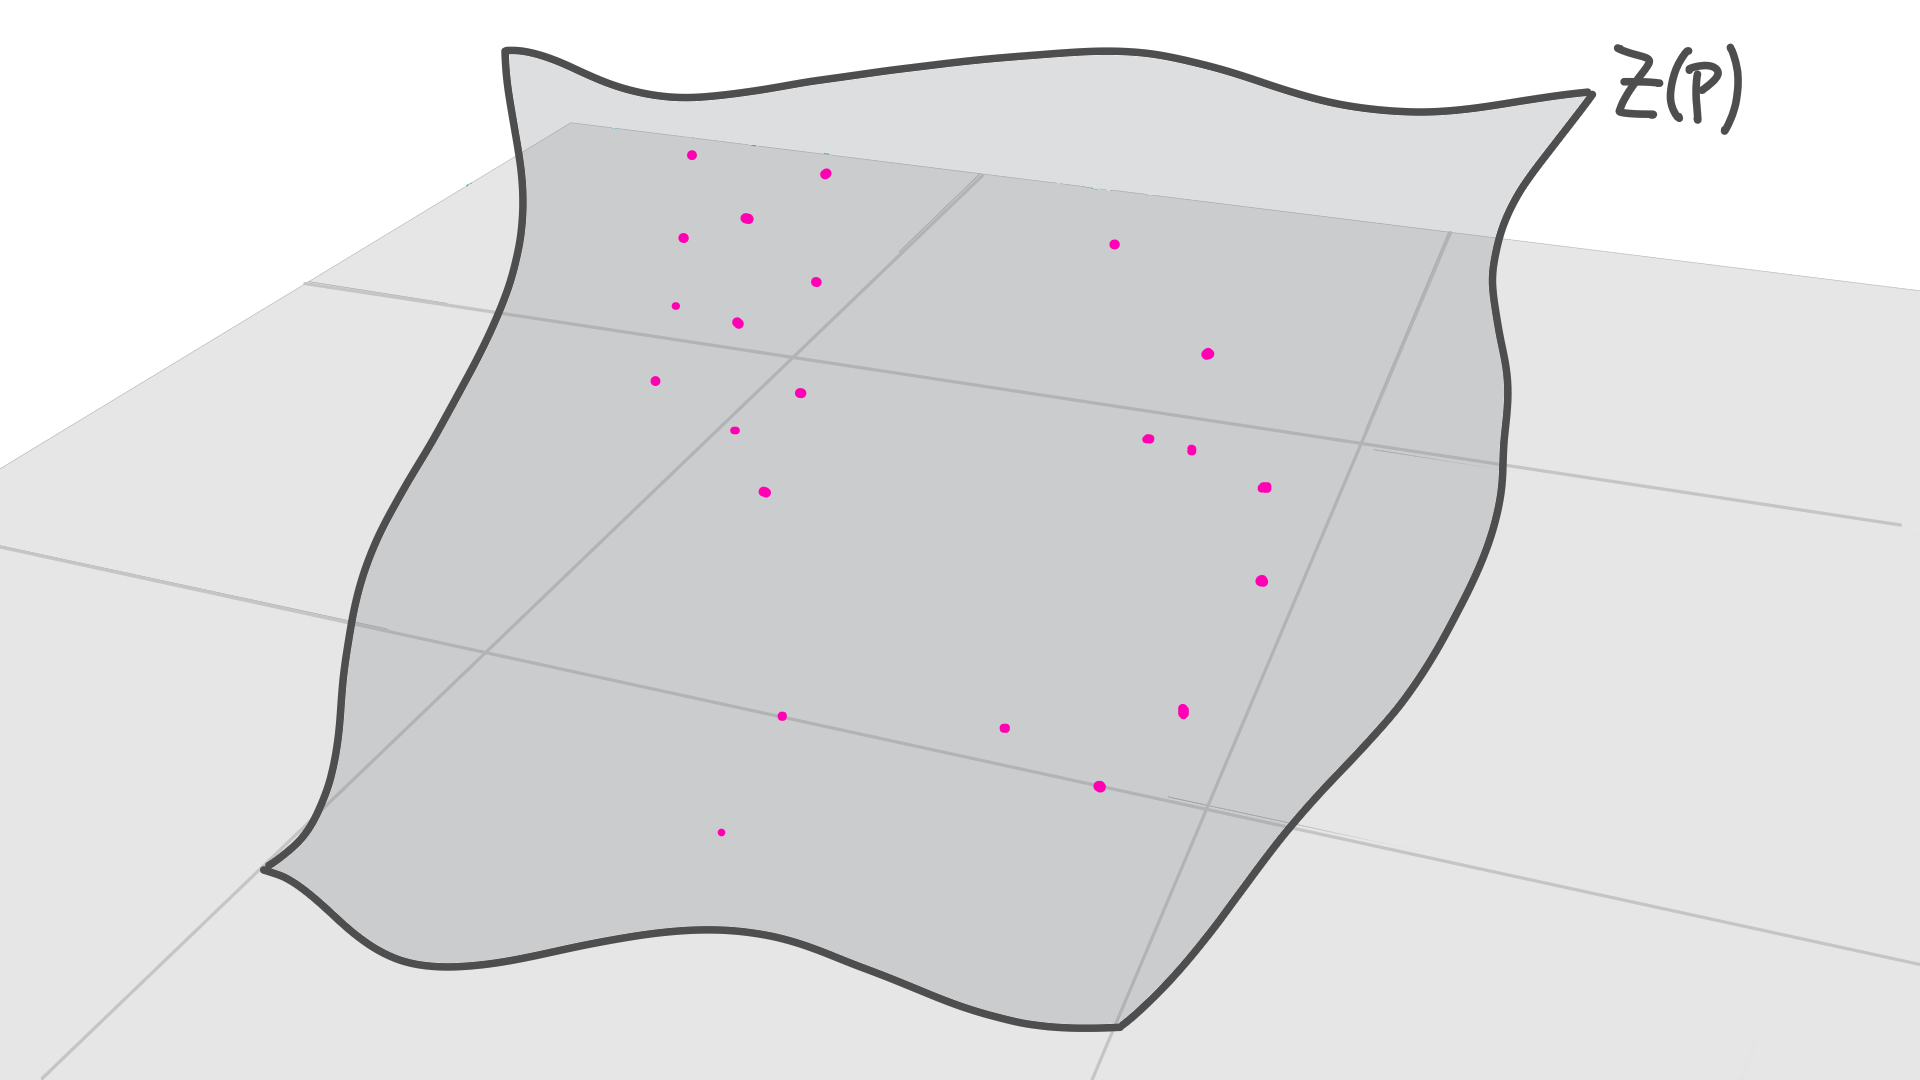
\includegraphics[width=0.7\textwidth]{images/lots_of_dots_c.png}
\end{figure} \pause
\begin{itemize}
    \item Recall that $\dim \RR_{\deg \leq D} [X,Y,Z] \sim D^3$. \pause
    \item Each incidence point gives one linear equation for the coefficients. \pause
    \item $D^3 \sim N^{3/2} \implies D \sim N^{1/2}$.
\end{itemize}

}

\nfr{{Circle Tangencies: $\beta(\gamma) \subset Z(P)$}
\begin{figure}[h]
    \centering
    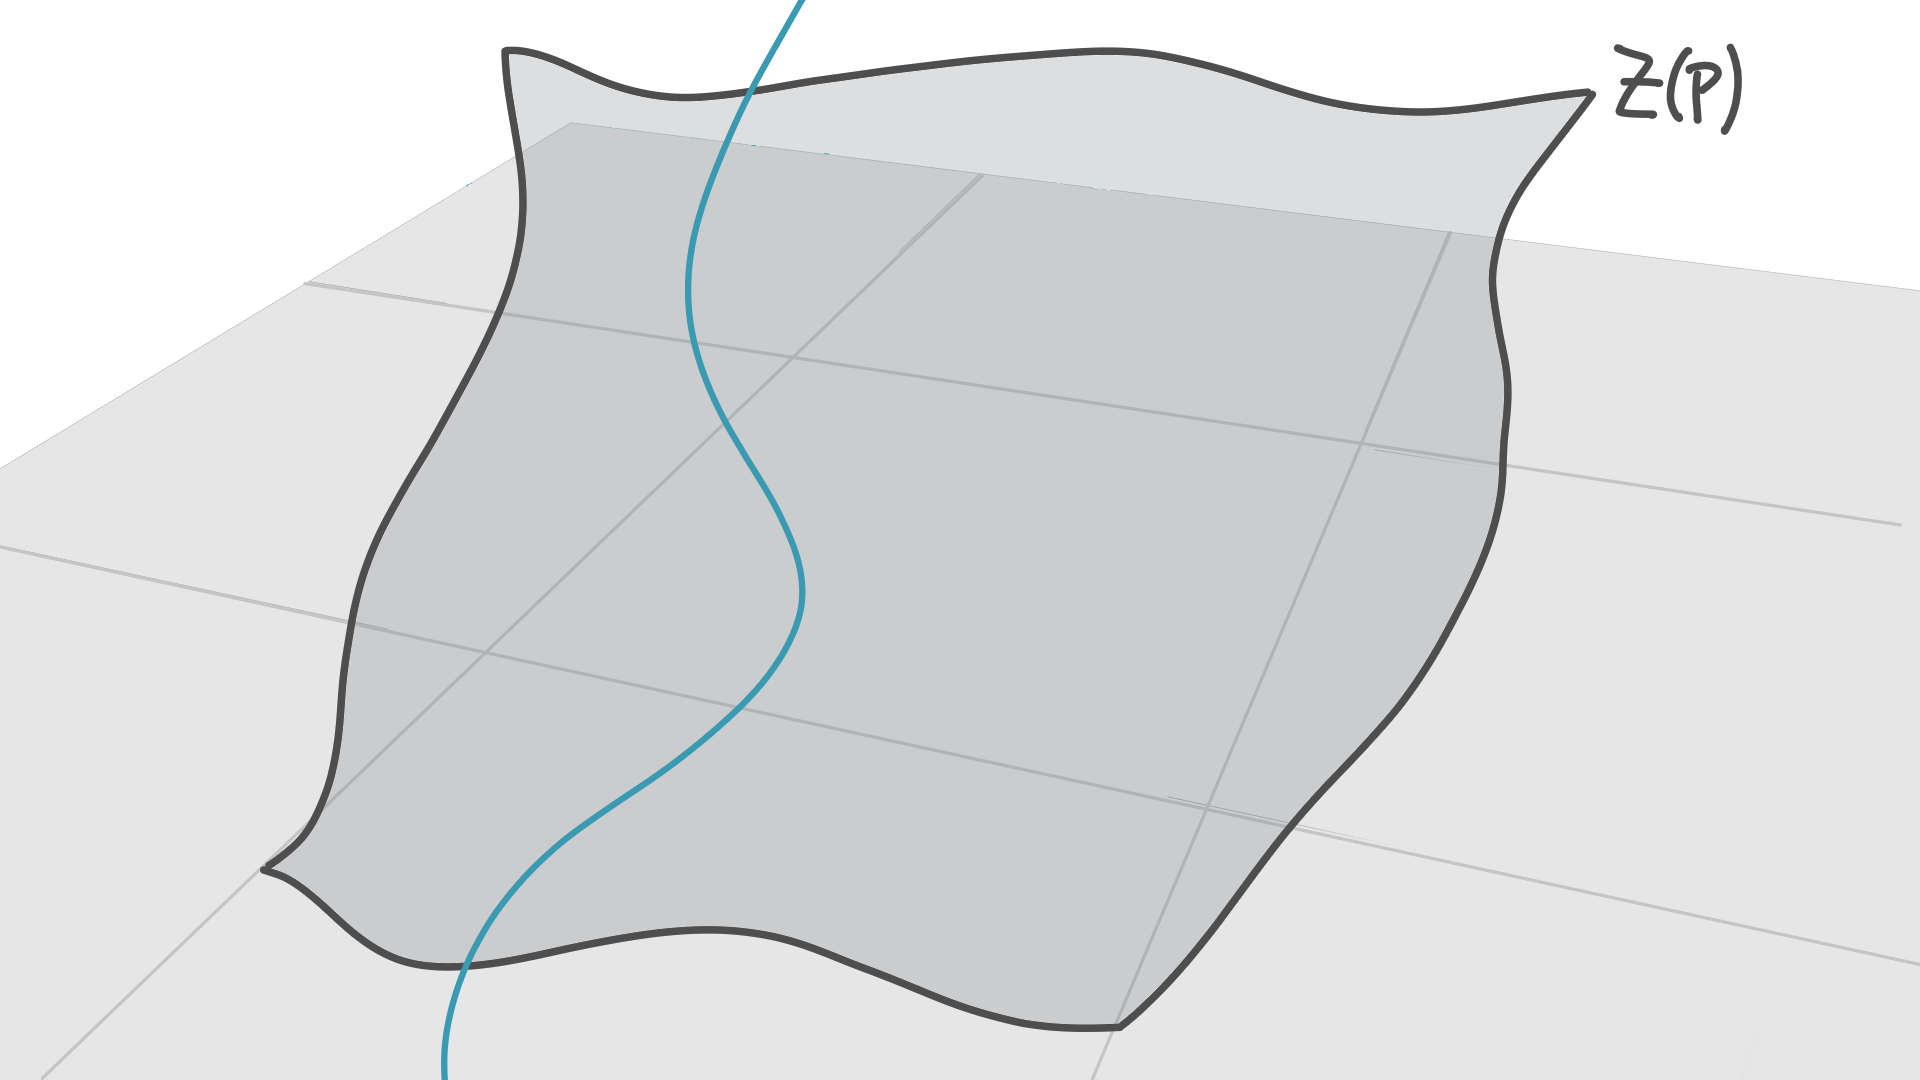
\includegraphics[width=0.7\textwidth]{images/lots_of_dots_e.png}
\end{figure}
}

\nfr{{Circle Tangencies: $\beta(\gamma) \subset Z(P)$}
\begin{figure}[h]
    \centering
    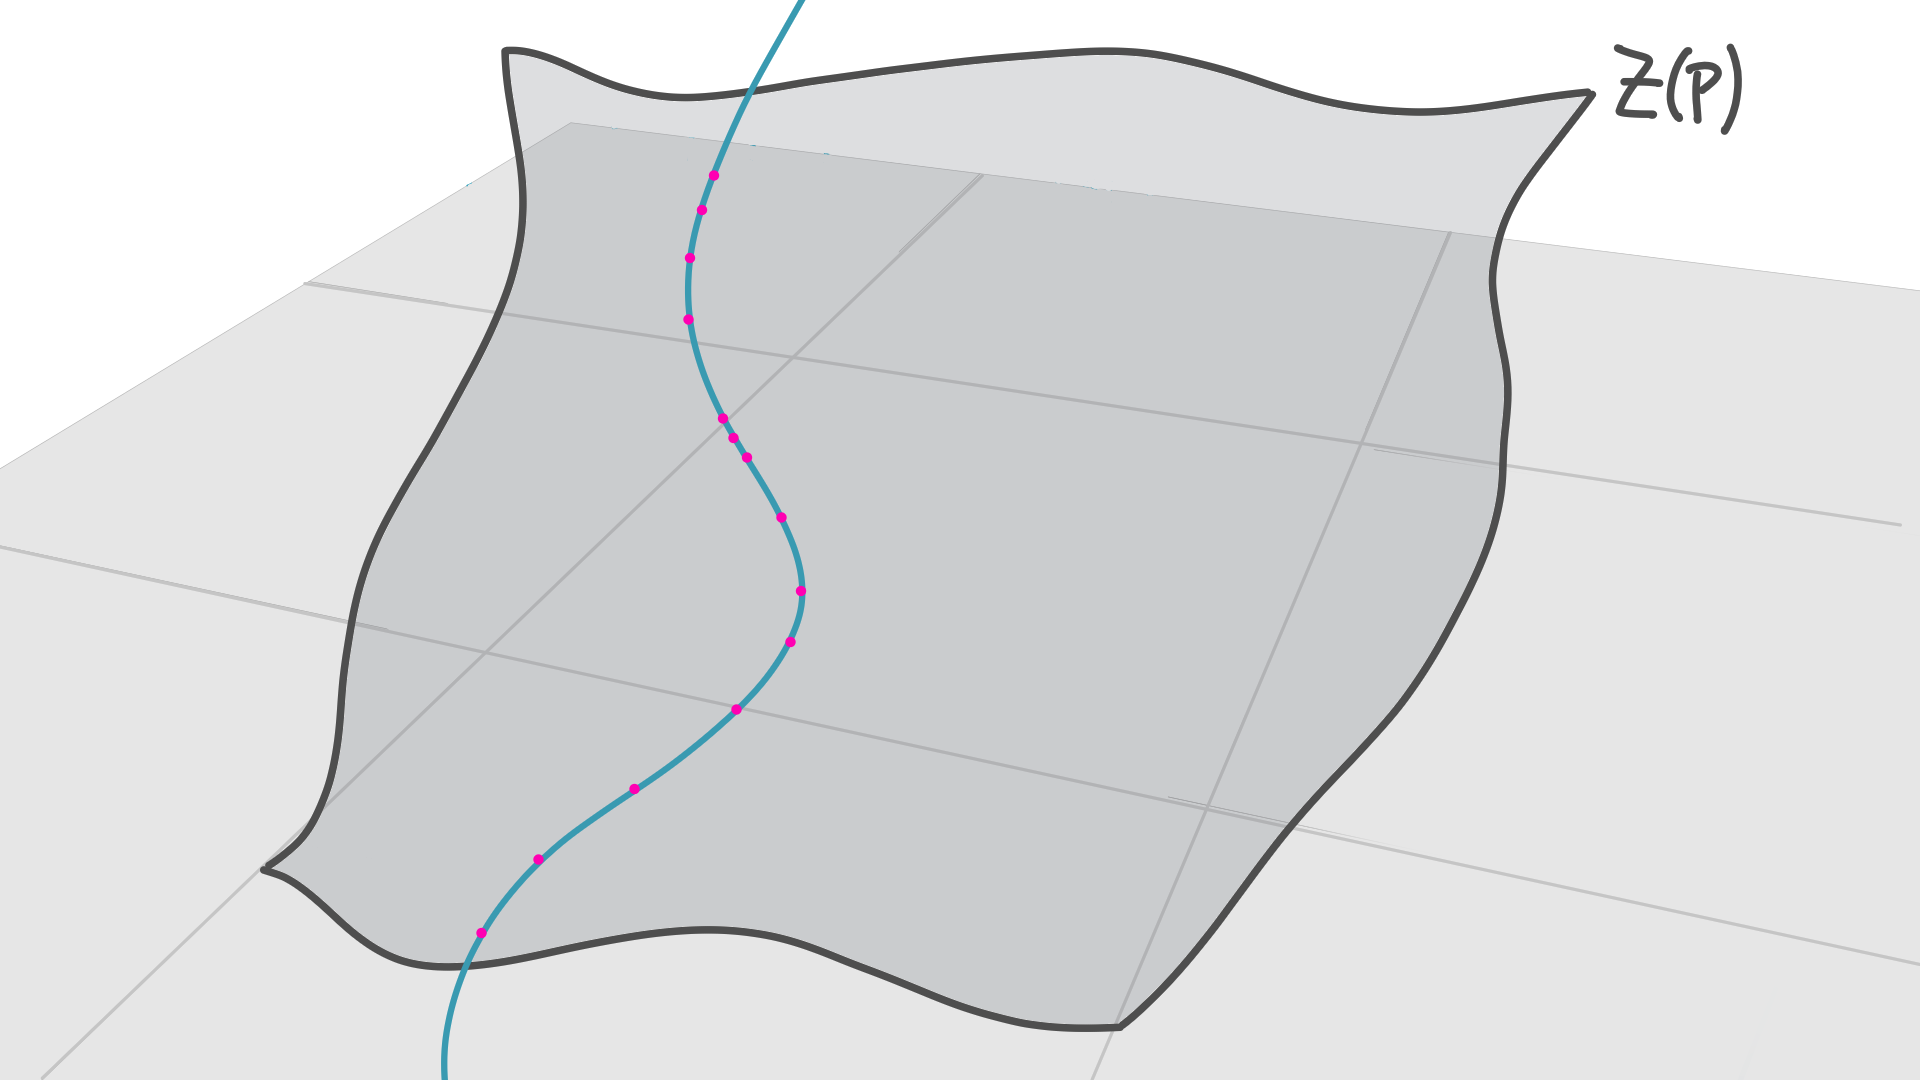
\includegraphics[width=0.7\textwidth]{images/lots_of_dots_f.png}
\end{figure}
\begin{itemize}
    \item Each curve $\beta(\gamma)$ intersects $Z(P)$ at $\gtrsim N^{1/2}$ points. \pause
    \item But $\deg \beta(\gamma) = O (1)$ and $\deg P \sim N^{1/2}$ \pause
    \item $\implies \beta(\gamma) \subset Z(P)$ by Bézout's Theorem! (rigidity)
\end{itemize}
}

\nfr{{Circle Tangencies: $\beta(\gamma) \subset Z(P)$}
\begin{figure}[h]
    \centering
    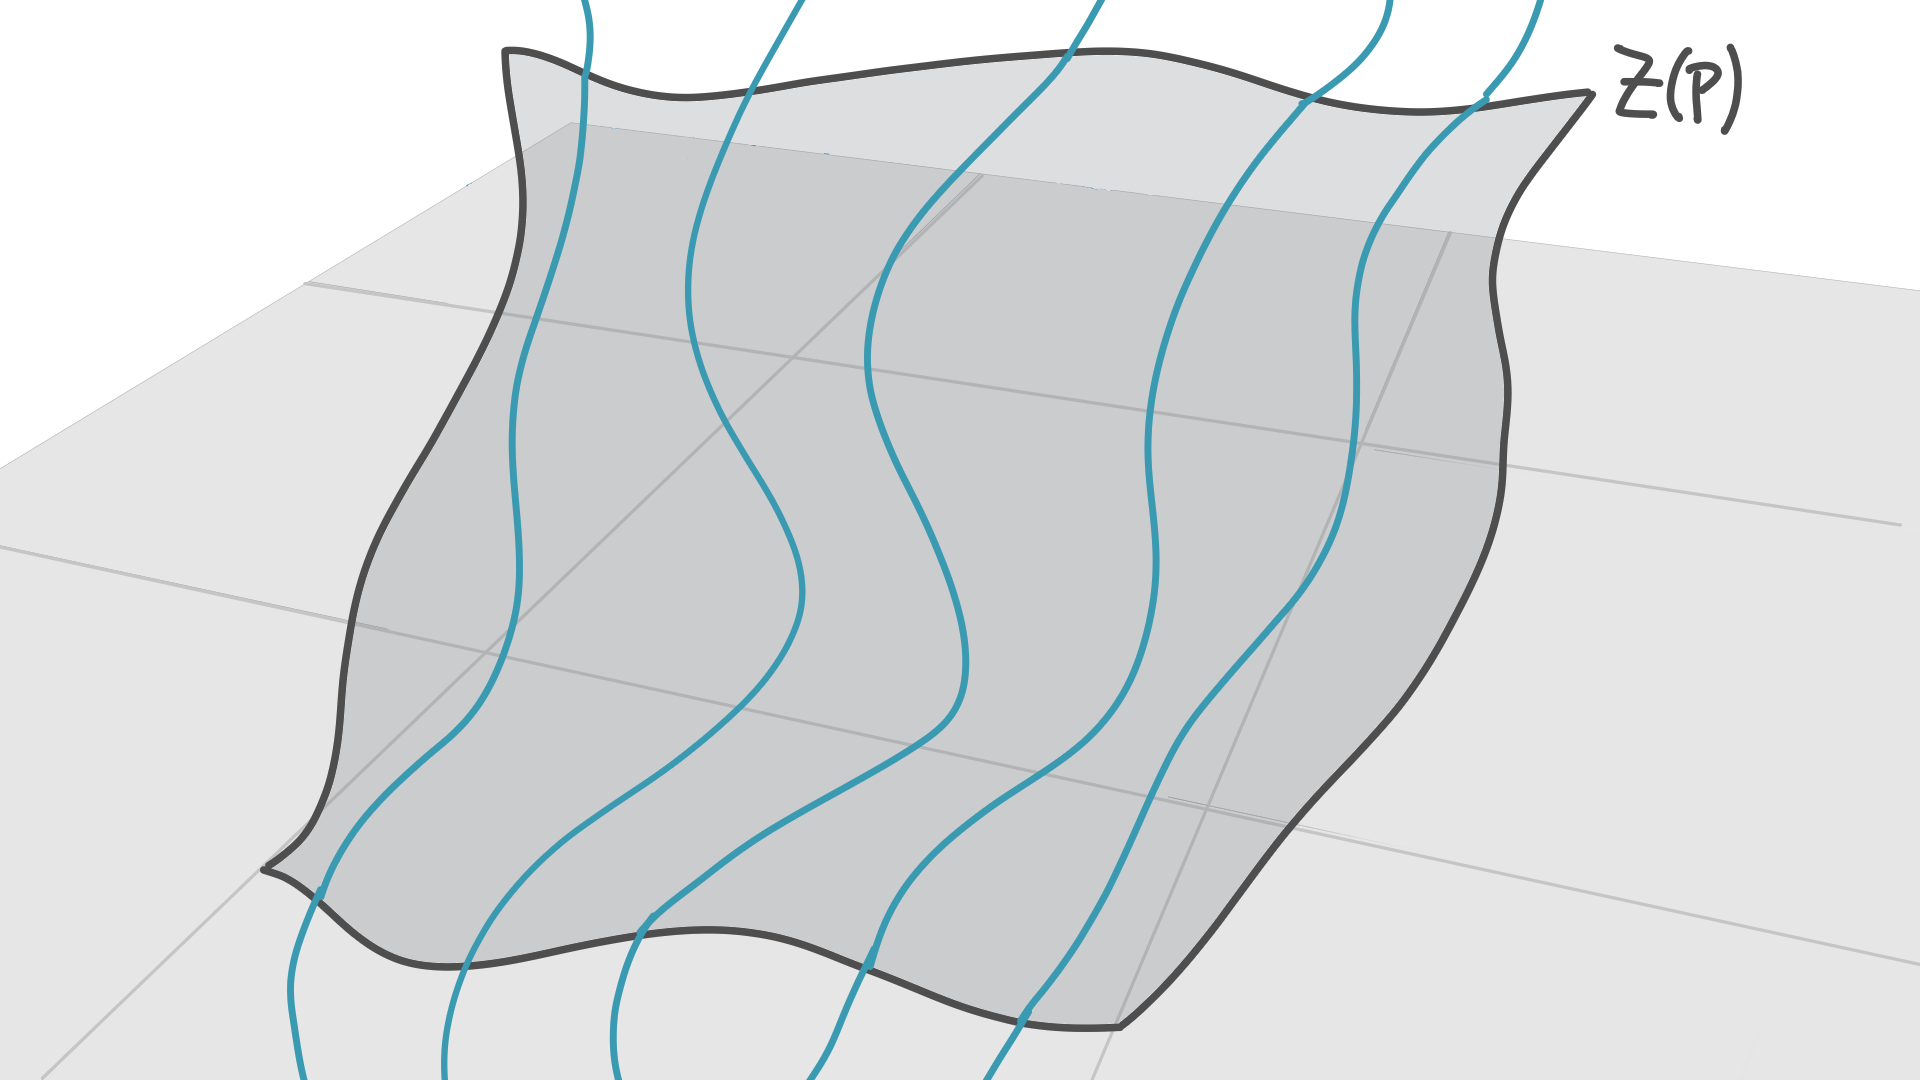
\includegraphics[width=0.7\textwidth]{images/lots_of_dots_g.png}
\end{figure}
\begin{itemize}
    \item Each curve $\beta(\gamma)$ contains $\gtrsim N^{1/2}$ points of intersection with $Z(P)$.
    \item $\deg \beta(\gamma) = O (1)$ and $\deg P \sim N^{1/2}$
    \item $\implies \beta(\gamma) \subset Z(P)$ by Bézout's Theorem.
\end{itemize}
}

\nfr{{Circle Tangencies: Tangent Vectors}
\begin{figure}[h]
    \centering
    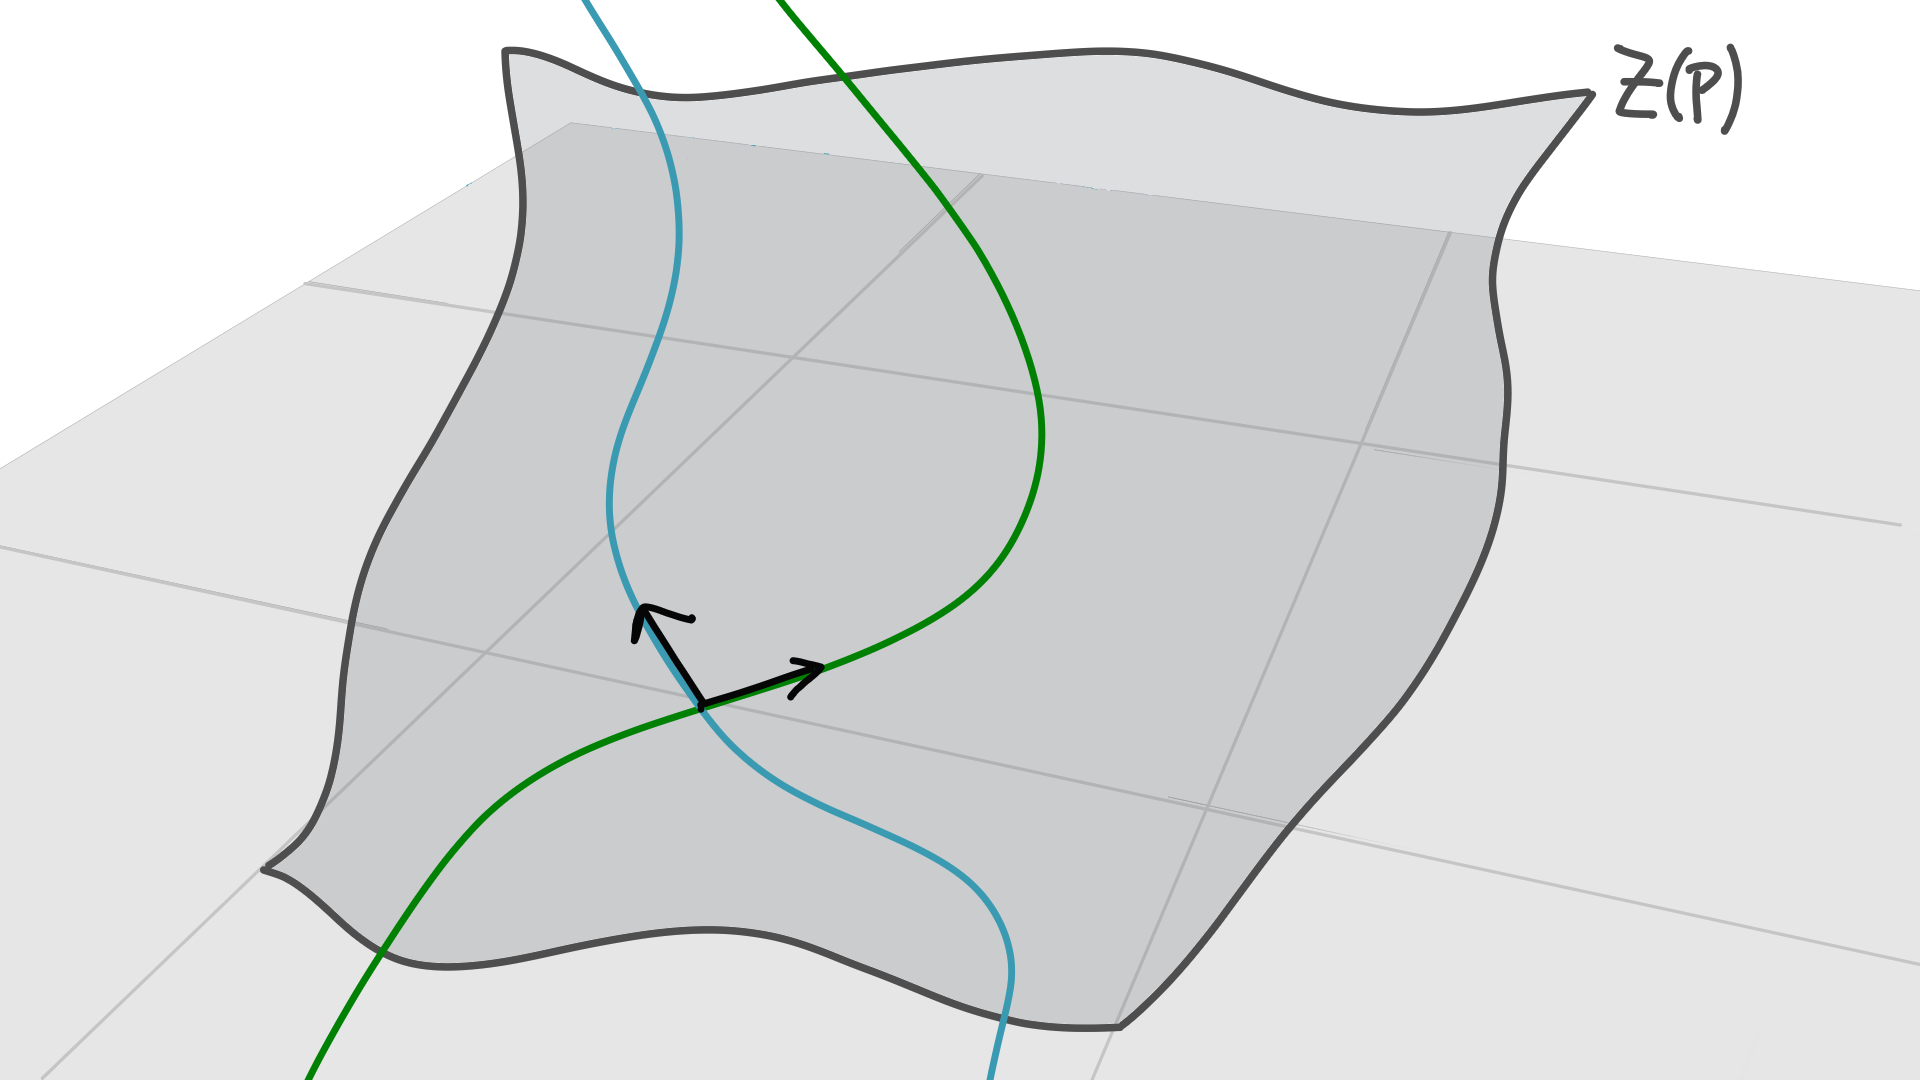
\includegraphics[width=0.7\textwidth]{images/lots_of_dots_h.png}
\end{figure}

}
\nfr{{Circle Tangencies: Tangent Vectors}
\begin{figure}[h]
    \centering
    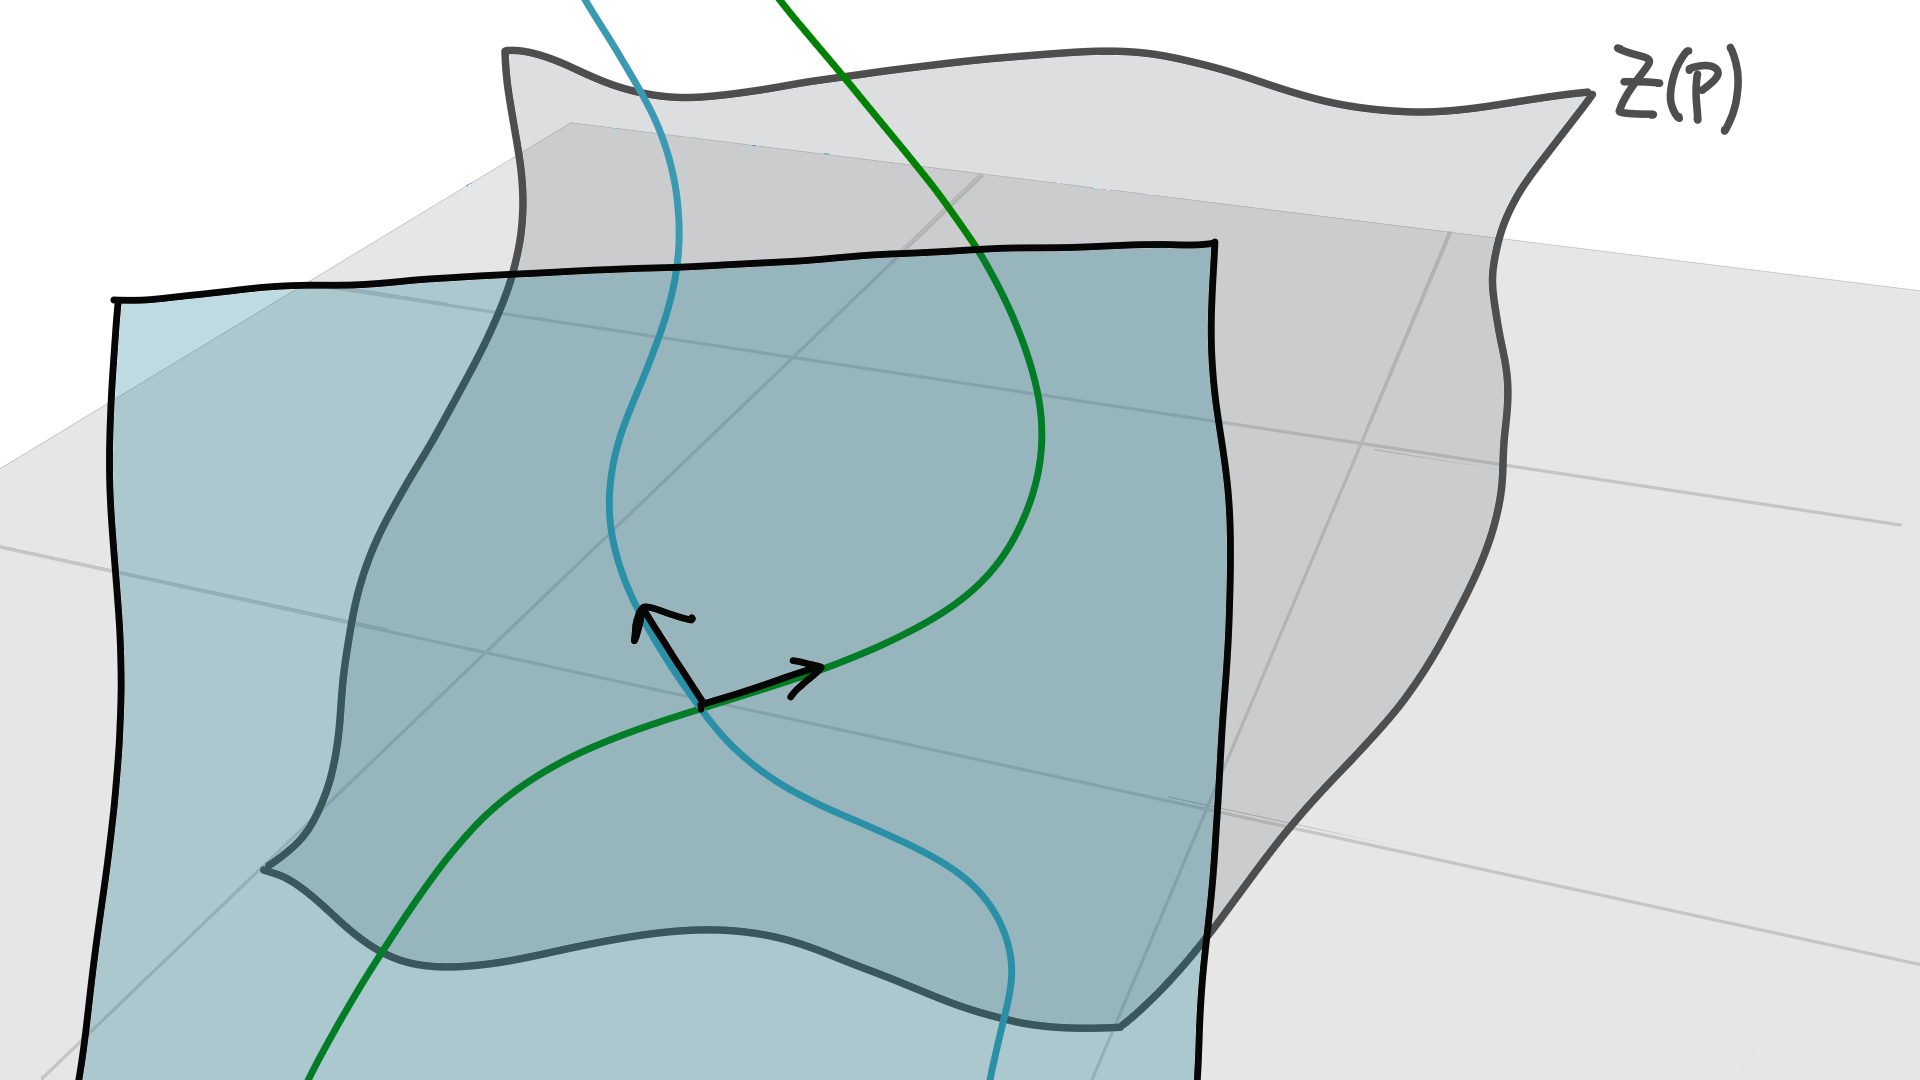
\includegraphics[width=0.7\textwidth]{images/lots_of_dots_i.png}
\end{figure}
\begin{itemize}
    \item Before we showed tangent space at incidences is vertical, so $\partial_z P = 0$ on all incidences! \pause
    \item $\implies Z(\partial_z P)$ also contains all incidences. \pause
    \item If $\deg P$ minimal $\implies P(X,Y,Z) = Q(X,Y)$.
\end{itemize}
}
\nfr{{Circle Tangencies: Contradiction}
\begin{figure}[h]
    \centering
    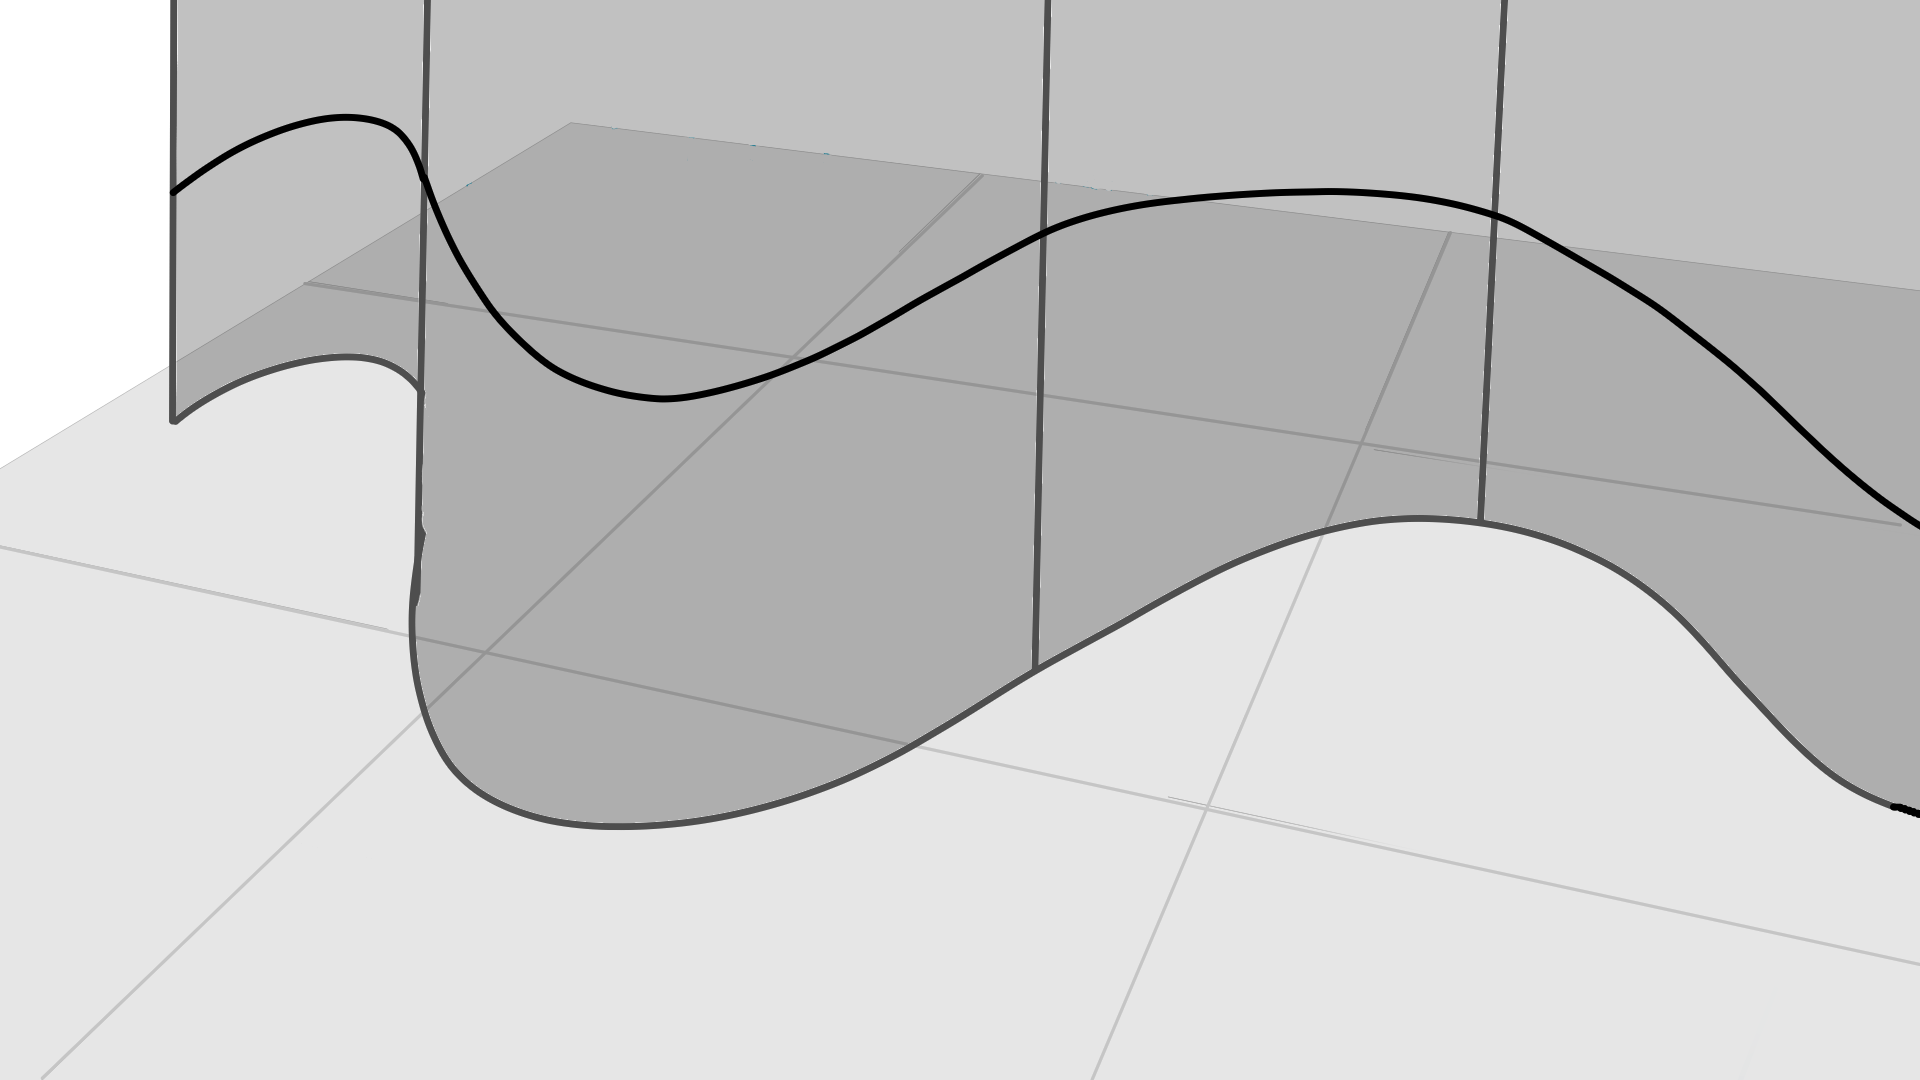
\includegraphics[width=0.7\textwidth]{images/lots_of_dots_j.png}
\end{figure}
Recall that $\deg P = \deg Q \sim N^{1/2}$, but $Z(Q)$ contains $N$ circles.
Contradiction!
}
\nfr{{Circle Tangencies: Recap of Argument}
\begin{theorem}
    Given a (suitably non-degenerate) collection of $N$ circles in $\RR^2$, they determine $\lesssim N^{3/2}$ tangencies.
\end{theorem}
\begin{enumerate}
    \item Assume there are $\gtrsim N^{3/2}$ tangencies.
    \item Lift curves into $\RR^3$ and change into an incidence problem.
    \item Use a low degree polynomial $P$ to interpolate these points. (parameter-counting)
    \item Argue that if $Z(P)$ contains $\gtrsim N^{1/2}$ points of $\beta(\gamma)$ then $\beta(\gamma) \subset Z(P)$. (rigidity)
    \item Use structure of the objects to argue $P(X,Y,Z) = Q(X,Y)$.
    \item Contradiction as degree of $Q$ is $\sim N^{1/2}$ but contains $N$ circles.
\end{enumerate}
}

\nfr{{Circle Tangencies: New Proof }
\begin{figure}[h]
    \centering
    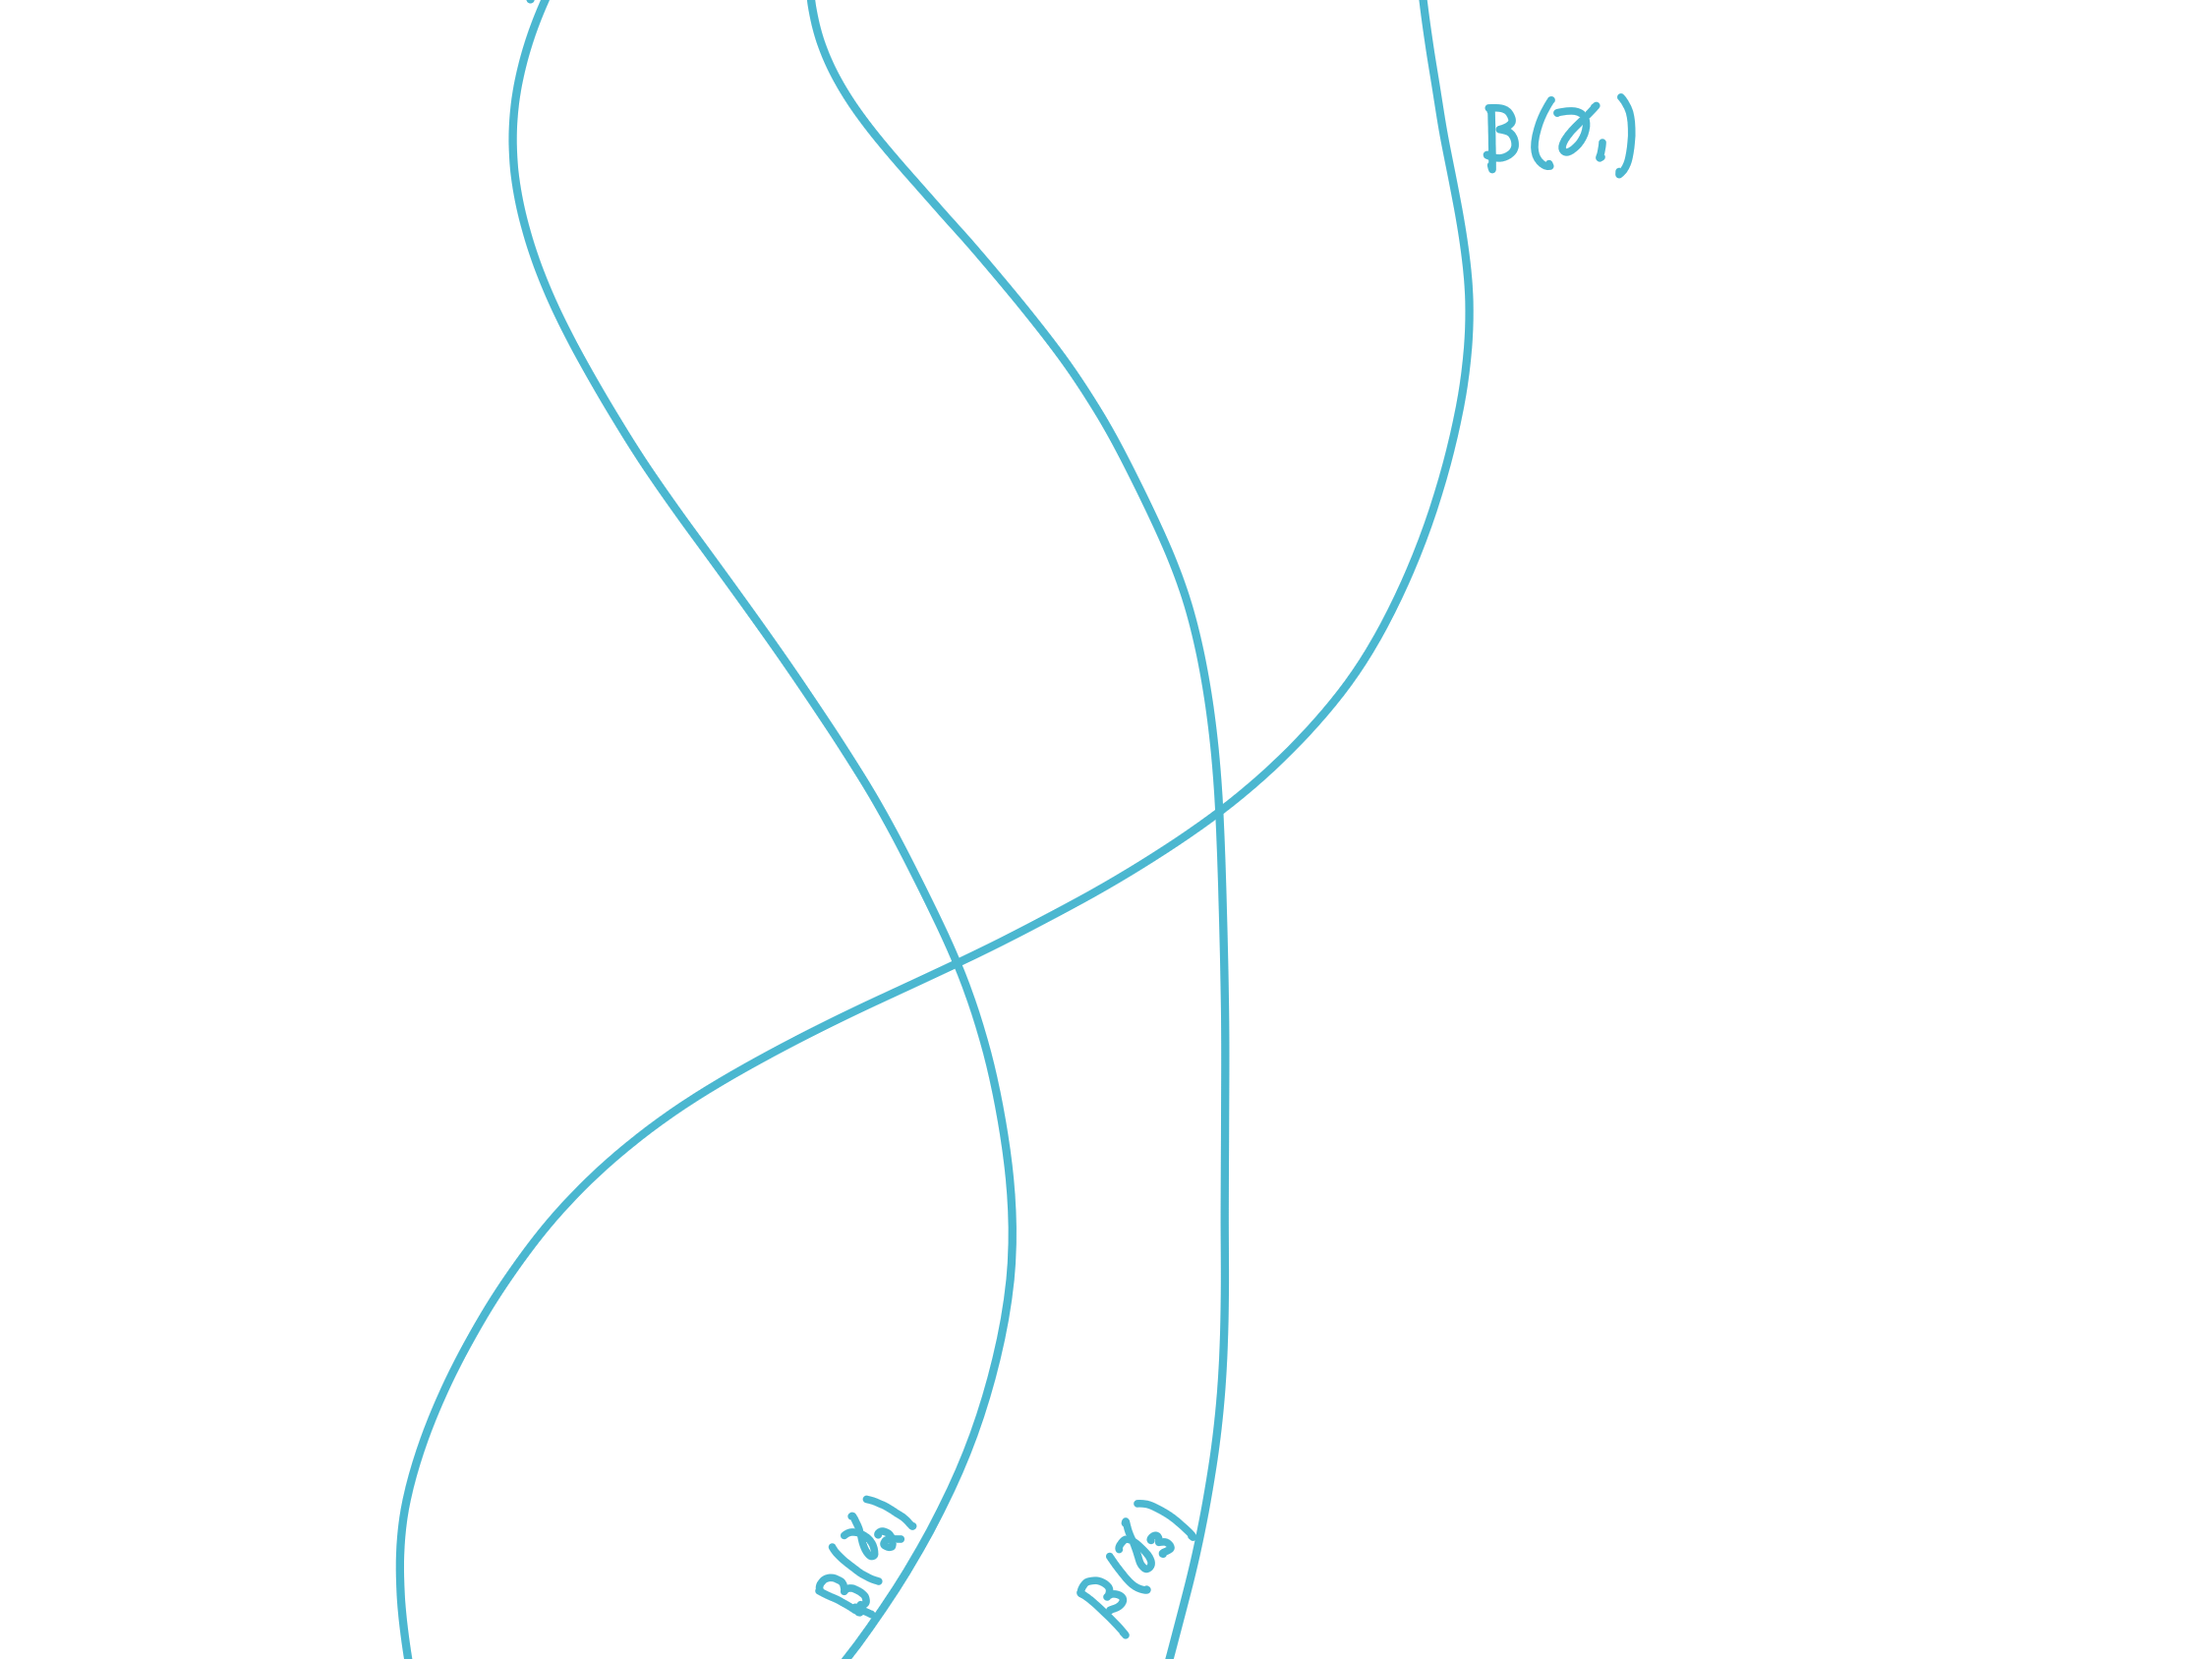
\includegraphics[width=0.6\textwidth]{images/new_proof_a.png}
\end{figure}
\textbf{Polynomial Partitioning:} We can find a polynomial $P$ of degree at most $D$ such that $Z(P)$ partitions $\RR^3$ into $\sim D^3$ cells such that each cell intersects $\lesssim \frac{N}{D^2}$ curves $\beta(\gamma)$.
}


\nfr{{Circle Tangencies: New Proof }
\begin{figure}[h]
    \centering
    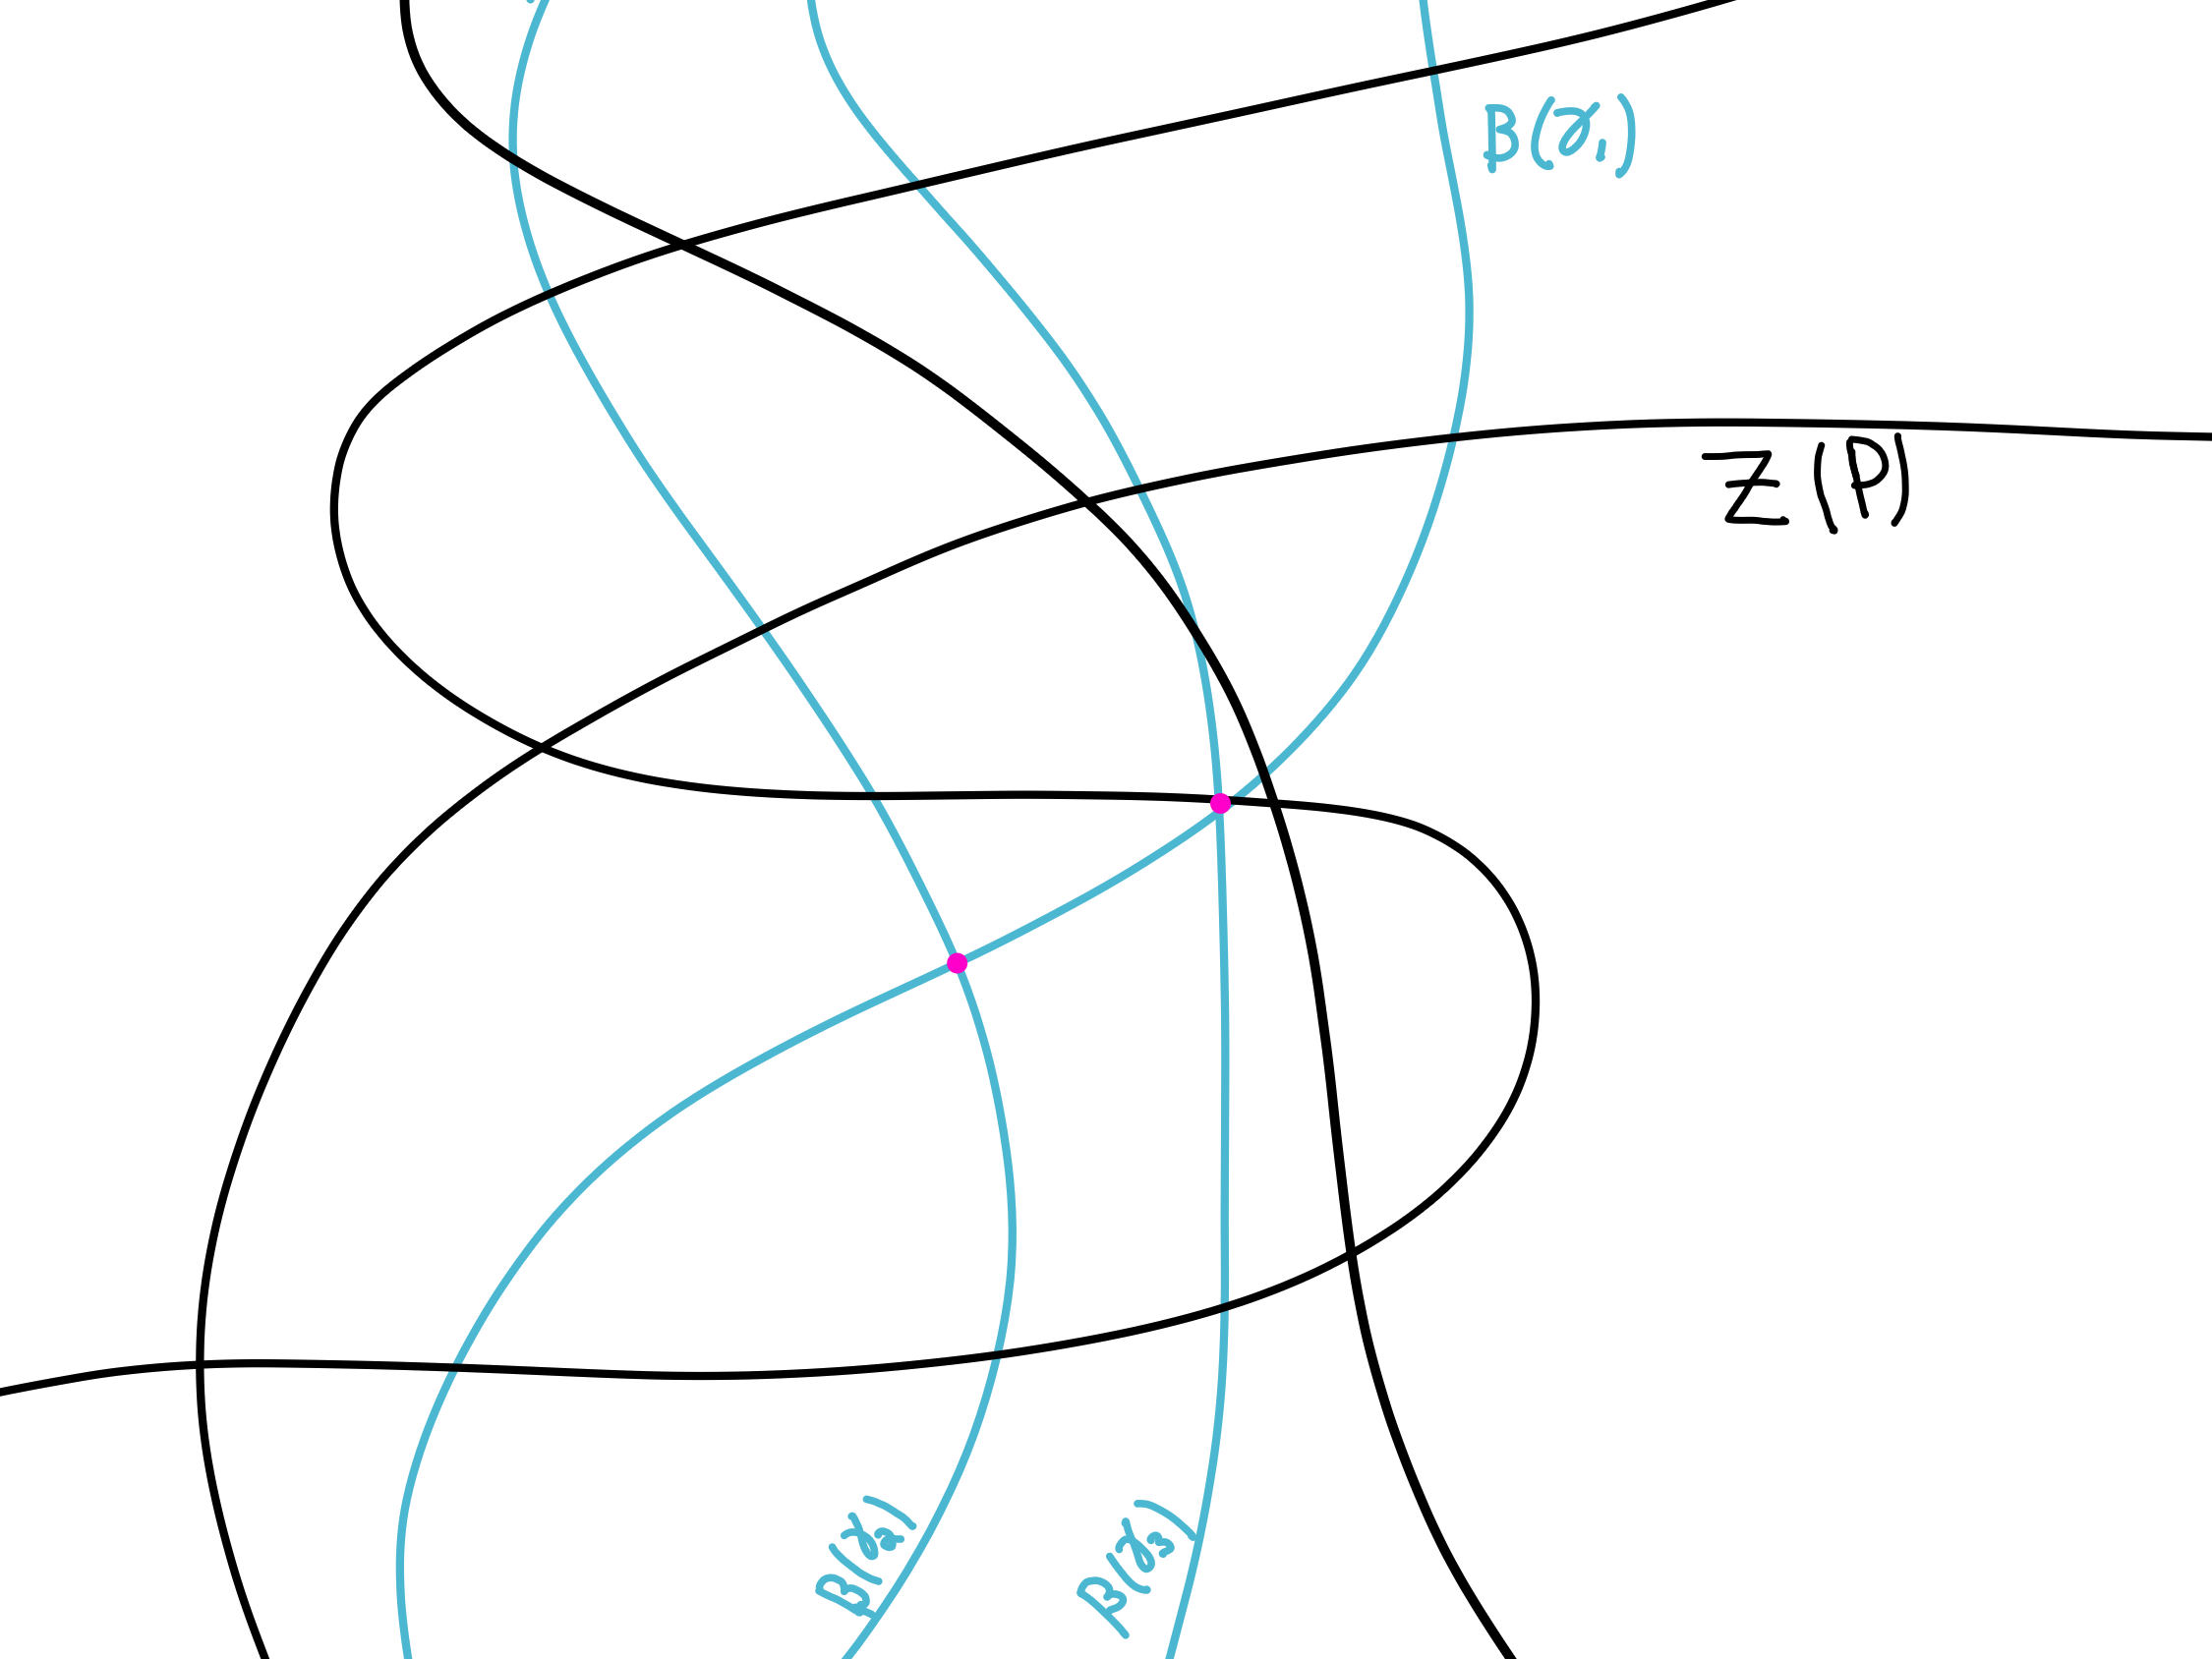
\includegraphics[width=0.6\textwidth]{images/new_proof_b.png}
\end{figure}
\textbf{Polynomial Partitioning:} We can find a polynomial $P$ of degree at most $D$ such that $Z(P)$ partitions $\RR^3$ into $\sim D^3$ cells such that each cell intersects $\lesssim \frac{N}{D^2}$ curves $\beta(\gamma)$.
}

\nfr{{Circle Tangencies: New Proof }
\begin{figure}[h]
    \centering
    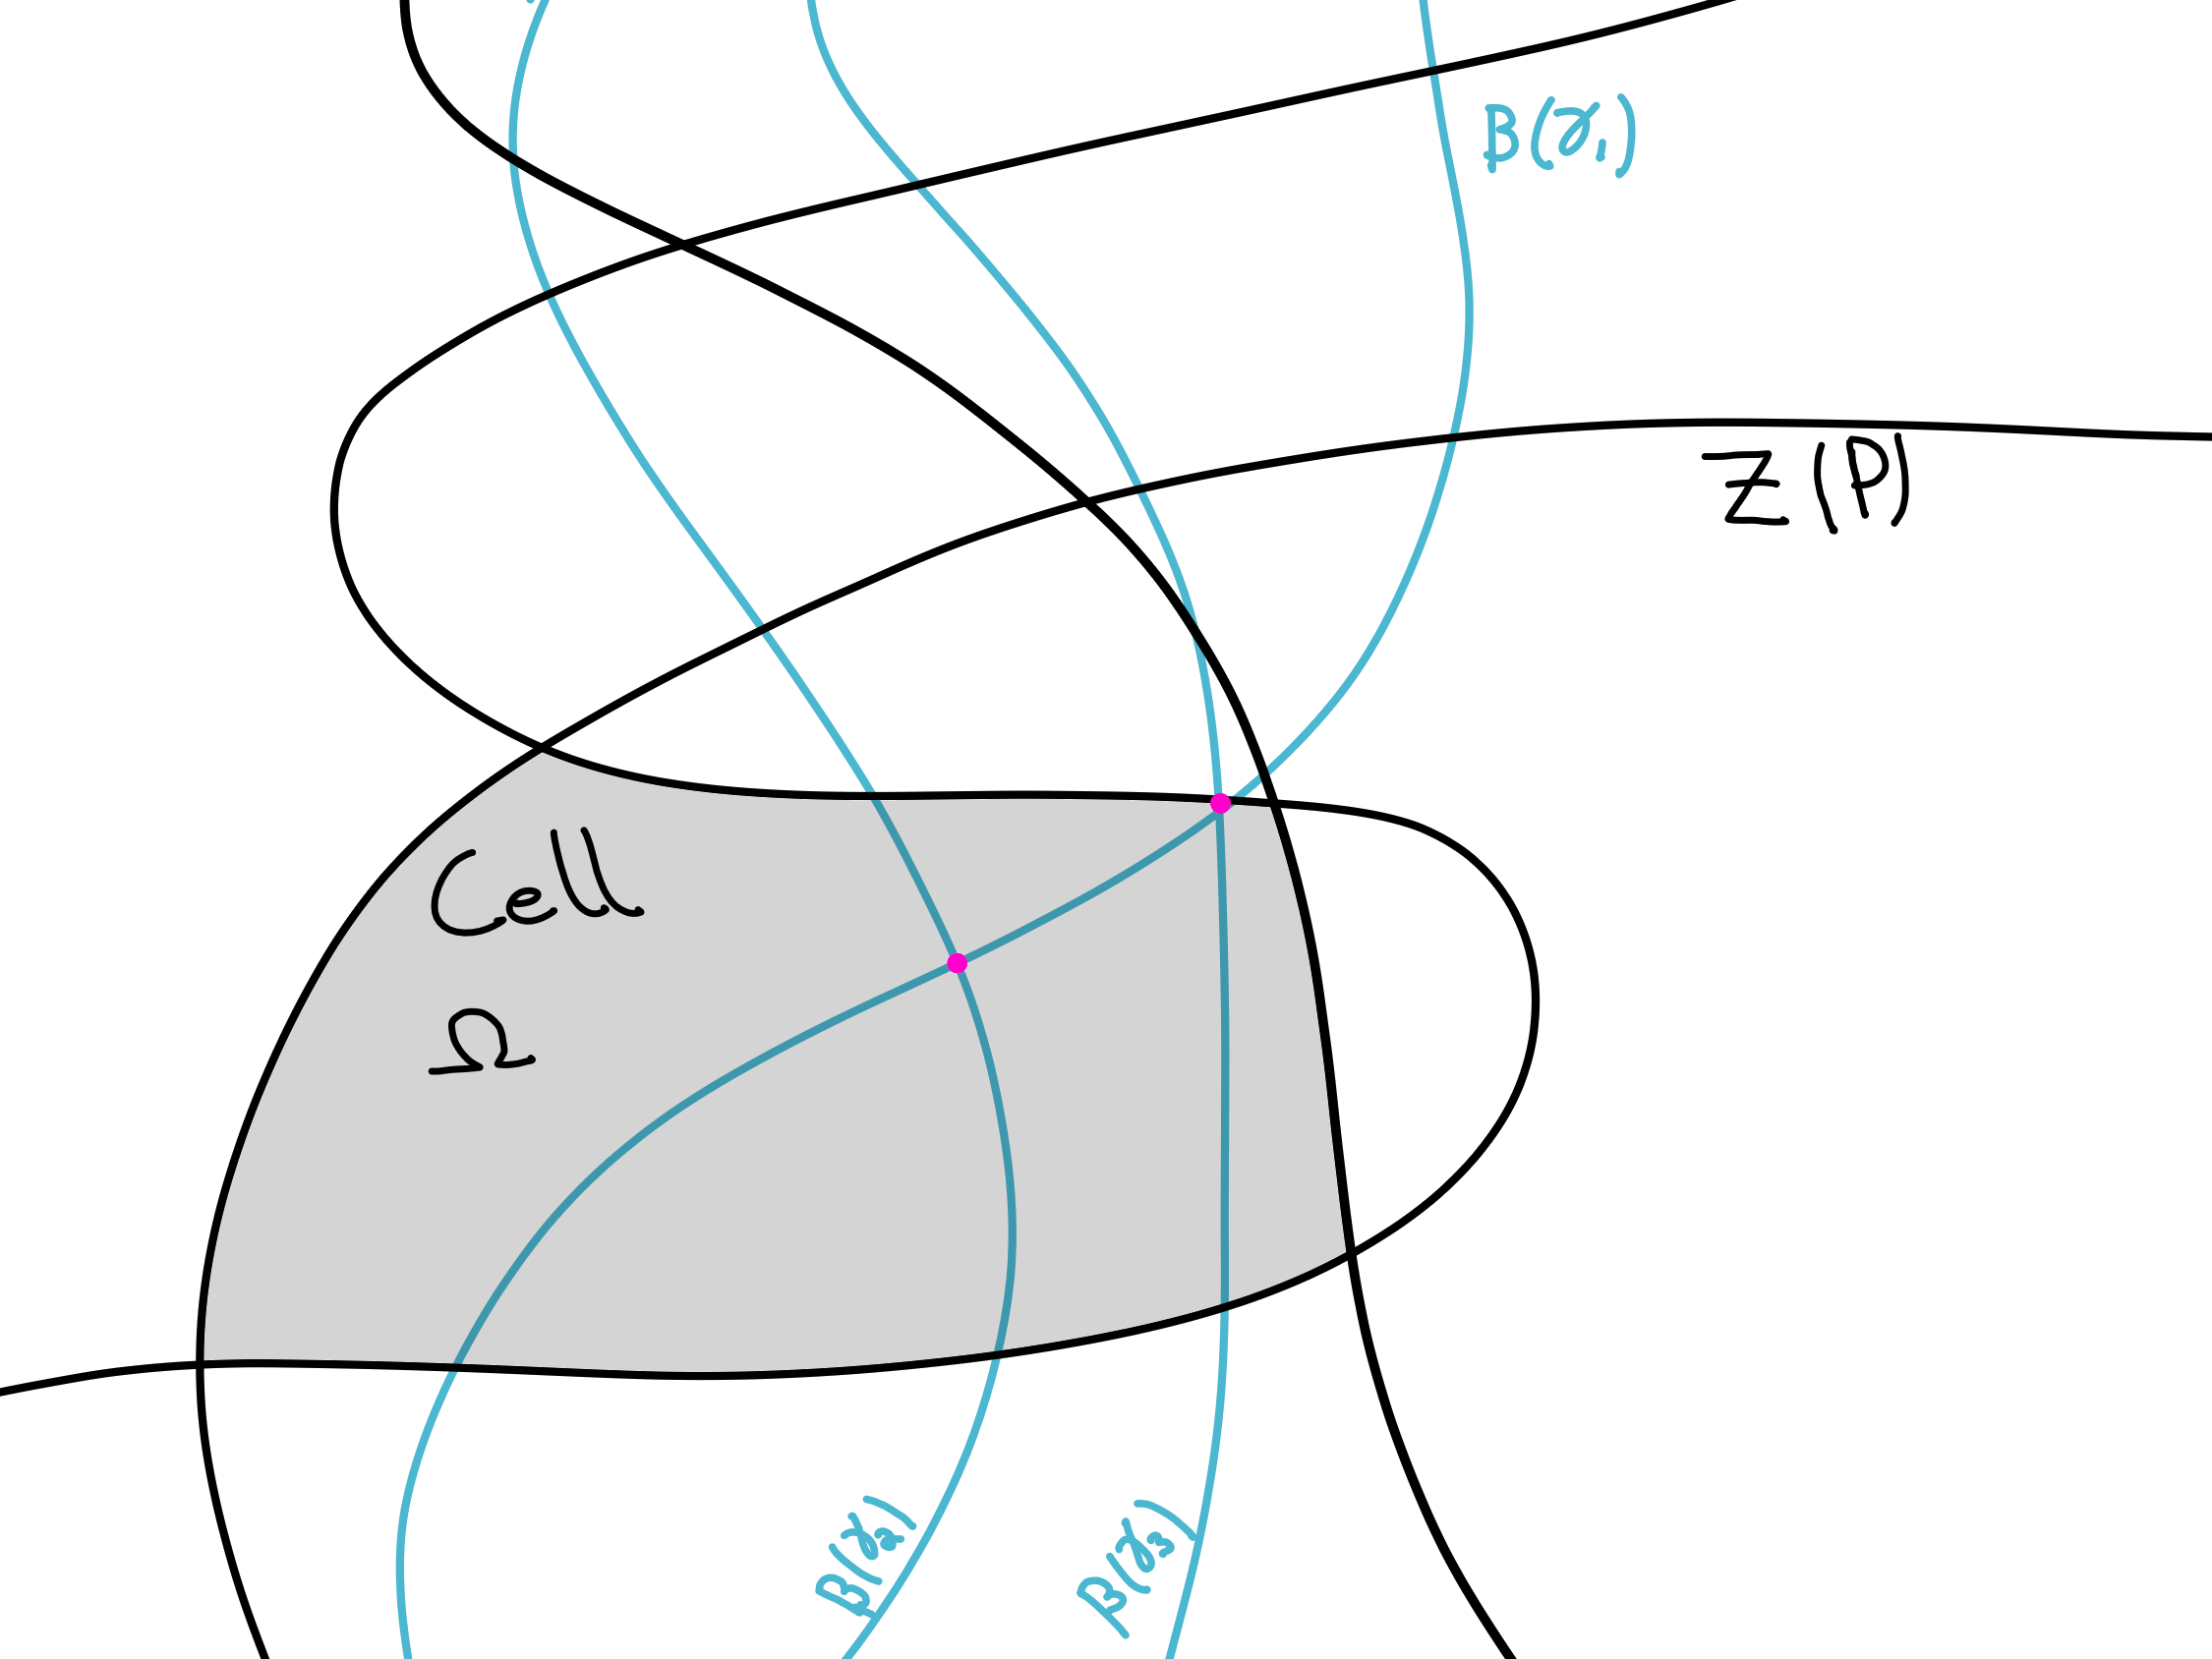
\includegraphics[width=0.6\textwidth]{images/new_proof_c.png}
\end{figure}
\textbf{Polynomial Partitioning:} We can find a polynomial $P$ of degree at most $D$ such that $Z(P)$ partitions $\RR^3$ into $\sim D^3$ cells such that each cell intersects $\lesssim \frac{N}{D^2}$ curves $\beta(\gamma)$.
}

\nfr{{Circle Tangencies: New Proof }
\textbf{Polynomial Partitioning:} We can find a polynomial $P$ of degree at most $D$ such that $Z(P)$ partitions $\RR^3$ into $\sim D^3$ cells such that each cell intersects $\lesssim \frac{N}{D^2}$ curves $\beta(\gamma)$.
Set of $\beta(\gamma)$'s can be partitioned:
\[
   C_1 = \{\beta(\gamma) \not \subset Z(P) \} \text{ and } C_2 = \{\beta(\gamma) \subset Z(P) \} 
\]
Total incidences of $\beta(\gamma)$'s = $I(C_1,C_1) +2I(C_1,C_2) + I(C_2,C_2)$  
}
\nfr{{Circle Tangencies: New Proof }
$I(C_1,C_1)$ = incidences between curves inside the cells. Each cell contains $\lesssim \frac{N}{D^2}$ curves so:
\[
  I(C_1,C_1) \leq \sum_{\text{cells}} \left(\frac{N}{D^2} \right)^2 
\]
\[
 = D^3 (N^2 D^{-4}) = N^2D^{-1}
\]
}

\nfr{{Circle Tangencies: New Proof }
$I(C_1,C_2)$ = incidences between a curve $\beta'$ in $Z(P)$ and a curve $\beta$ not in $Z(P)$.
\[
    I(C_1,C_2) = \sum_{\beta \in C_1} \sum_{\beta' \in C_2} \OO[\beta \cap \beta' \neq \emptyset]
\]
Each $\beta(\gamma) \in C_1$ can intersect $Z(P)$ at most $\lesssim D$ times. (Bézout)
\[
\lesssim  \sum_{\beta \in C_1} D \lesssim ND
\]
}

\nfr{{Circle Tangencies: New Proof }
$I(C_2,C_2)$ = incidences between $\beta(\gamma)$'s both in $Z(P)$. 
We can assume $P$ was of minimal degree for the partitioning.
We consider $\partial_z P$:

\textbf{Case 1:} $Z(\partial_z P)$ contains all the curves of $C_2$. Proceed by same argument in previous proof to yield a bound of $\lesssim ND$.

\pause
\textbf{Case 2:} $C_2 \backslash Z(\partial_z P)$ is non-empty. There are $\lesssim D$ incidences between curves in $C_2 \backslash Z(\partial_z P)$ and the zero set. 
We repeat the process up to $D$ times until we are in case 1, accumulating $ \lesssim \sum D = D^2$ incidences.
}

\nfr{{Circle Tangencies: New Proof }
Adding these up we get the number of tangencies to be:
\[
    I(C_1,C_1) +I(C_1,C_2) + I(C_2,C_2) \lesssim N^2 D^{-1} + ND + D^2  
\]
\pause
We optimize $D$ now by setting $N^2 D^{-1} \sim ND \implies D \sim N^{1/2}$.

We achieve:
\[
    \lesssim  N^{3/2} 
\]
}

\nfr{{Circle Tangencies: Recap of New Proof}

\begin{enumerate}
    \item Lift curves into $\RR^3$ and change into an incidence problem.
    \item Use a low degree polynomial $P$ to partition $\RR^3$ into $D^3$ cells, each intersecting $\lesssim ND^{-2}$ curves. (parameter-counting + Borsuk-Ulam)
    \item Use a trivial bound in each cell and sum over all cells.
    \item Deal with curves contained in the zero set using algebraic tools. 
    \item Choose $D$ to optimise inequality and achieve $\lesssim N^{3/2}$ bound.
\end{enumerate}
}
\nfr{{}
\begin{center}
Thank you for your attention.

Any questions? 

\end{center}
}


\bibliographystyle{unsrt}
\bibliography{slides}

\end{document}